\section{Finden von ähnlichen Hotels}
\label{sec:find_similar}
Das finden von ähnlichen Hotels ist die Grundlage dieses Konzeptes. Um dies zu erreichen soll das vorgehen, welches in der Sektion \emph{\nameref{sec:aehnliche_hotels}} beschrieben wurde, verfolgt werden. Angefangen mit der Datenbeschaffung, muss sich zunächst ein überblick darüber gemacht werden, welche Daten schon vorhanden sind und welche Daten gegeben falls noch besorgt werden müssen, bevor dann mit der Datenanalyse und der Modellierung weiter gemacht werden kann. 

\subsection{Datenbeschaffung}
\label{subsec:Datenbeschaffung}
Durch die verschiedenen Property Management Systeme sind für die einzelnen Hotels bereits Stammdaten wie Zimmeranzahl oder Zimmerkategorien vorhanden. Zudem wird der jeweilige Kunde beim Einrichten von happyhotel auch schon nach verschiedenen Daten befragt. Unter den Daten, die bei einem Kunden abgefragt werden, gehören Informationen wie zum Beispiel die Adresse des jeweiligen Hotels. 
\newline
\newline
Werden nun alle schon vorhanden Informationen zusammengetragen, die bisher in der Datenbank zur Verfügung stehen, entsteht dabei das folgende Dataframe:
\begin{figure}[h]
    \centering
    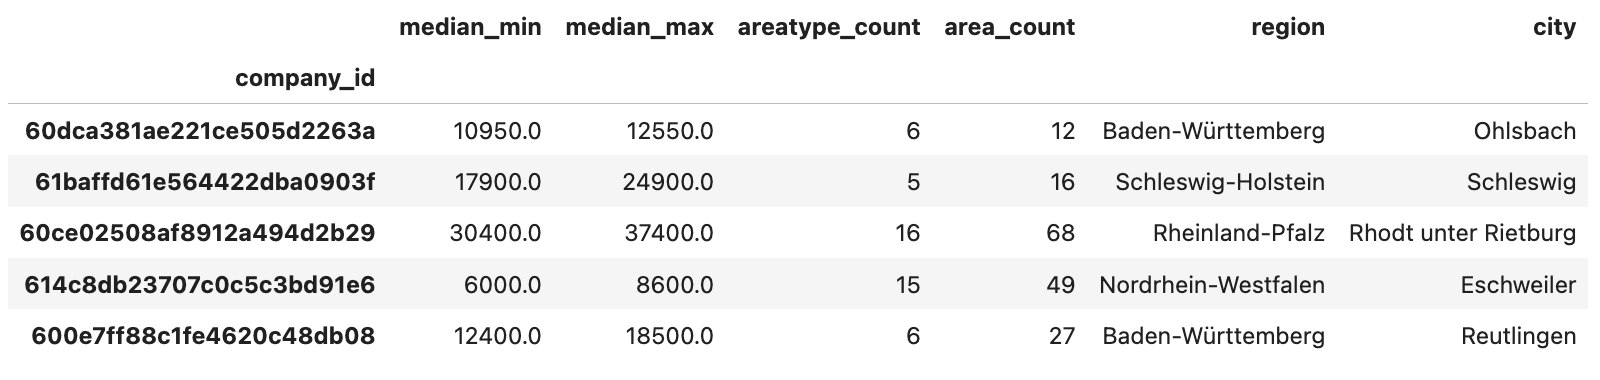
\includegraphics[width=1\textwidth, center]{Features_1.png}
    \caption[Alle schon vorhanden Features]{Alle schon vorhanden Features}
    \label{img:all_Features}
\end{figure}

In Abbildung \ref{img:all_Features} sind die Daten zu sehen, die bislang zur Verfügung stehen, wobei sich die \emph{median\_min} und \emph{median\_max} Werte auf den Median aller Zimmerkategorie-Preise bezieht.
\newline
\newline
Dadurch, dass \emph{region} und \emph{city} manuell vom Kunden eingetragene Werte sind, ergab sich eine gewisse Skepsis, ob alle Werte norm-konform eingetragen wurden. Aufgrund dieser Skepsis sollte eine kleine Datenanalyse getätigt werden. 
\newline
\newline
Bei der Datenanalyse wurde jeweils nach der Region und nach der Stadt gruppiert, um zu prüfen ob die Daten so benutzt werden können. Im Folgenden sind die Werte jeweils für die Region und für die Stadt zu sehen:

\begin{figure}[h]
    \centering
    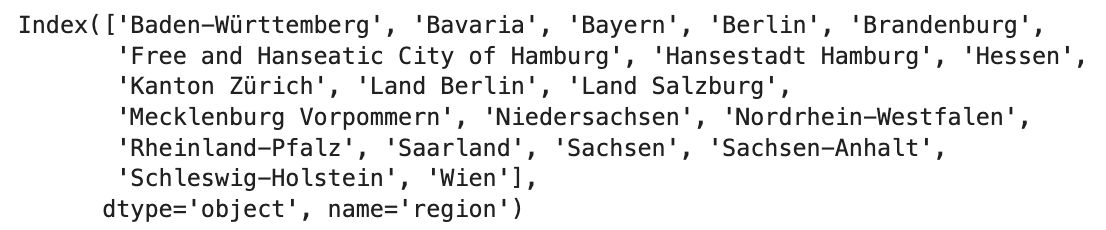
\includegraphics[width=0.8\textwidth, center]{region_1.png}
    \caption[Alle vorhanden Regionen]{Alle vorhanden Regionen}
    \label{img:region_1}
\end{figure}

\begin{figure}[h]
    \centering
    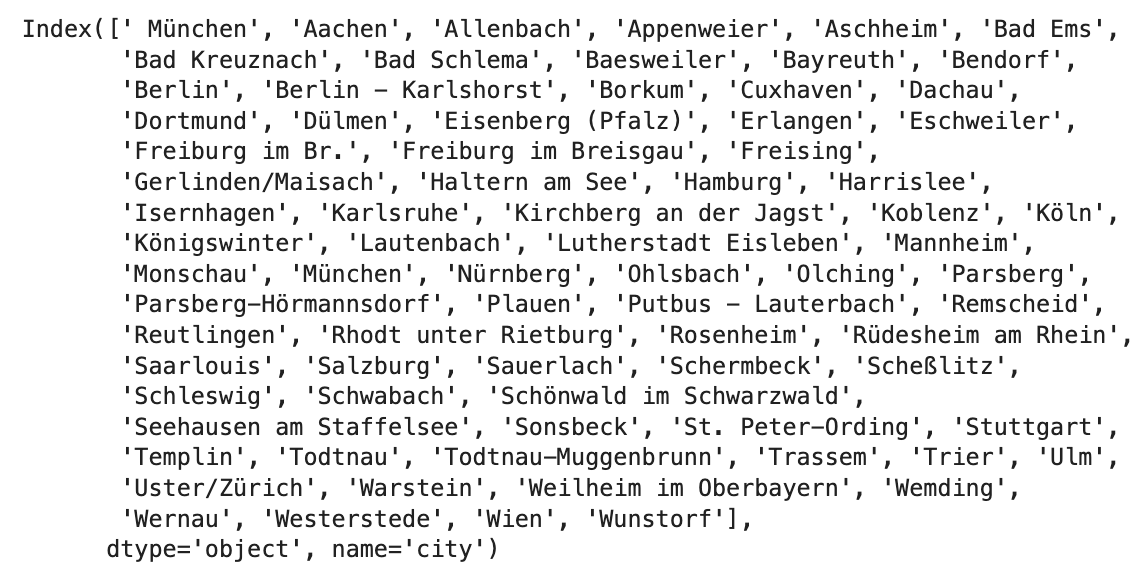
\includegraphics[width=0.8\textwidth, center]{city_1.png}
    \caption[Alle vorhanden Städte]{Alle vorhanden Städte}
    \label{img:city_1}
\end{figure}

Es ist eindeutig zu erkennen, dass es sowohl bei der Region als auch bei der Stadt zu einer Inkonsistenz kommt. So wurde die Region \emph{Berlin} sowohl als \emph{Berlin}, als auch mit \emph{Land Berlin} angegeben. Auch bei der Stadt ist die Diskrepanz deutlich zu erkennen, -so wurde bspw. \emph{München} mit Leerzeichen vorne dran angegeben oder die Stadt Freiburg einmal mit der Abkürzung \emph{Br.} und ein anderes Mal mit komplett ausgeschriebenen \emph{Breisgau} angegeben. Es ergab sich also, dass diese Werte so wie sie sind, nicht verwendet werden können.

\subsubsection{Beschaffung von Region, City und Stadtgröße}
\label{subsubsec:region_city_size}
Durch eine schon im Vorfeld getätigte Arbeit, existiert zu jedem Hotel in unserer Datenbank, die Koordinaten, repräsentiert durch die zwei Werte Long- und Latitude. Mithilfe von diesen zwei Werten sollte ein Skript geschrieben werden um die Region, die Stadt und Größe der Stadt zu beschaffen. 
\newline
\newline
Für das Skript wurde \emph{Nominatim} API verwendet um die einzelnen Werte zu beschaffen. Im folgenden wird das Skript präsentiert:

\begin{lstlisting}[language=Python, label=lst:RS_Demo, caption=Einfaches Recommendation System für Film vorschläge]
    from geopy.geocoders import Nominatim

def get_region_city_size(latitude, longitude):
    geolocator = Nominatim(user_agent="city_size_app")
    location = geolocator.reverse((latitude, longitude), language='de')

    address = location.raw['address']

    if 'city' in address:
      region = address["city"]
      if 'state' in address:
        region = address["state"]
      return {
            "city": address["city"],
            "region": region,
            "size": "Großstadt"
        }
    elif 'town' in address:
        return {
            "city": address["town"],
            "region": address["state"],
            "size": "Kleinstadt"
        }
    elif 'village' in address:
      region = None
      if 'county' in address:
        region = address["county"]
      if 'state' in address:
        region = address["state"]
      return {
            "city": address["village"],
            "region": region,
            "size": "Kleinstadt"
        }
    else:
        return dict()
\end{lstlisting}

Die Funktion \emph{get\_region\_city\_size} nimmt als Parameter die Long- und Latitude Werte und erzeugt dadurch ein \emph{Dictionary} mit den Werten \emph{region}, \emph{city} und \emph{size}.
\subsubsection{Beschaffung von der Hotelart}
\label{subsubsec:hotelart}
Einer der wichtigsten Eigenschaften, die ein Hotel vorweisen kann, ist die Hotelart von dem jeweiligen Hotel. Die Hotelart hängt maßgeblich mit der zur grundlegenden Preisgestaltung ab. Dies ist einfach zu erklären, da Hotels existieren, die eher auf Wellness ausgelegt sind und somit prinzipiell teurer sind als einfache Urlaubshotels. Somit ist die Art eines Hotels essentiell um ähnliche Hotels zu finden. So soll auch für das Modell die Hotelart vorhanden sein. Dieses Feature muss jedoch erst beschafft werden, da diese Information nicht in der Datenbank hinterlegt ist. 
\newline
\newline
Leider ist der Versuch, die Hotelart auf einem automatisiertem Weg zu bekommen, gescheitert und es blieb nichts anderes übrig als die Hotelart eines jedem Hotels manuell herauszufinden. 
\newline
\newline
Nachdem die Hotelart beschaffen wurde, sieht der Feature-Datensatz wie folgt aus:
\begin{figure}[h]
    \centering
    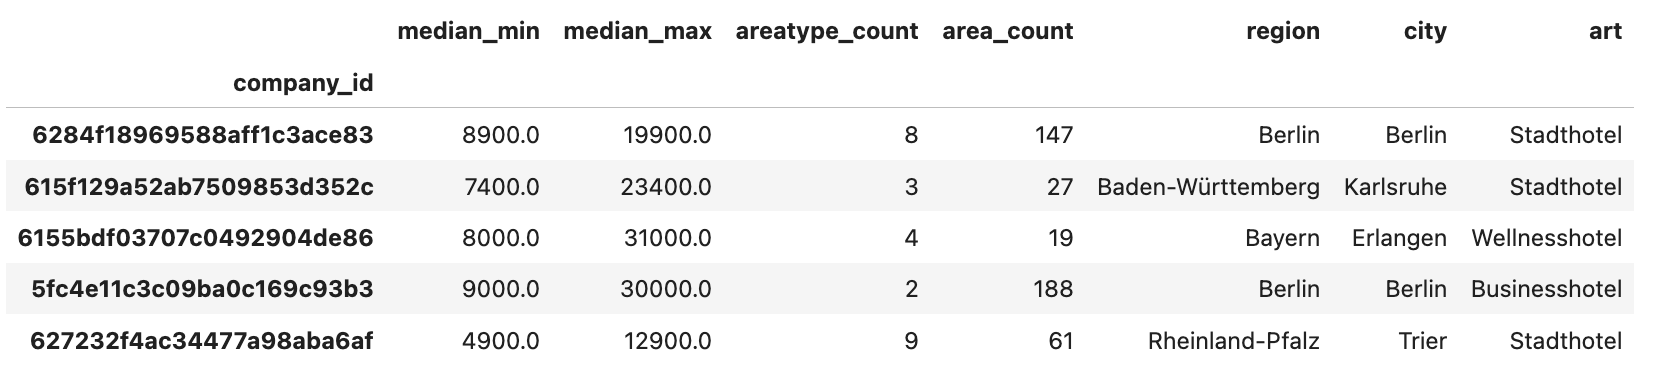
\includegraphics[width=1\textwidth, center]{Features_2.png}
    \caption[Alle schon vorhanden Features #2]{Alle schon vorhanden Features #2}
    \label{img:all_Features_2}
\end{figure}

\subsection{Datenvorverarbeitung}
\label{subsec:Datenvorverarbeitung}
Nach der Datenbeschaffung erfolgt die Datenvorverarbeitung, die darauf abzielt, die Qualität und Integrität der Daten sicherzustellen. Ein zentraler Schwerpunkt liegt dabei auf der Identifikation und Eliminierung fehlerhafter oder ungültiger Datensätze. Häufig wird innerhalb der Datensätze nach Nullwerten gesucht, um diese entweder durch valide Daten zu ersetzen oder in einigen Fällen gänzlich zu entfernen. Im vorliegenden Fall ist es Wichtig, dass sämtliche als verwendbar gekennzeichneten Hotels in die Analyse einbezogen werden. Die Datensätze sollen nicht einfach verworfen werden; vielmehr erfolgt eine gezielte Substitution von Nullwerten durch valide Daten, um eine konsistente und zuverlässige Grundlage für die weiterführende Analyse zu gewährleisten \cite{Agarwal.05.10.2018}.
\newline
\newline
Im folgenden ist die Anzahl aller Nullwerte innerhalb des Datensatzes zu sehen:
\begin{figure}[h]
    \centering
    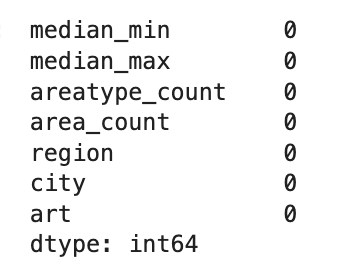
\includegraphics[width=0.4\textwidth, center]{Null_values.png}
    \caption[Summe aller Nullwerte im Datensatz]{Summe aller Nullwerte im Datensatz}
    \label{img:null_values}
\end{figure}

In Abbildung \ref{img:null_values} ist zu sehen, dass innerhalb des es Datensatzes keine Nullwerte gibt und somit auch keine Datenvorverarbeitung getätigt werden muss.
\subsection{Allgemeine Datenanalyse}
\label{subsec:Datenanalyse}
Die Datenanalyse ist ein, wenn nicht sogar der Wichtigste schritt im Data Science Bereich \cite{Agarwal.05.10.2018}. Dabei sollen die Daten ergründet und verstanden werden. Dieser Schritt soll nicht nur ein Verständnis für die vorliegenden Daten schaffen, sondern auch \emph{outlier} erfassen. Meist wird auch versucht innerhalb der Datenanalyse zusammenhänge zu der Zielvariable zu finden. Dies setzt jedoch voraus, dass eine Zielvariable vorhanden ist. In dem vorliegenden Fall existiert keine Zielvariable, da nicht bekannt ist welche Hotels mit welchen Hotels ähnlich sind. Aufgrund dessen, dass keine Zielvariable vorhanden ist, wird die folgende Datenanalyse lediglich dazu genutzt um die Daten besser zu verstehen. Zudem soll festgestellt werden, welche Daten wie als Features verwendet werden können.
\newline
\newline
Für die Datenanalyse soll die Python-Bibliothek \emph{Seaborn} benutzt werden. Die \emph{Seaborn}-Bibliothek stellt ein leistungsstarkes Werkzeug dar, das speziell für die Erstellung von statistischen Grafiken in Python entwickelt wurde \cite{Melanie.2023}. Das Hauptziel besteht darin, die verschiedenen Verteilungen der Features auf anschauliche Weise darzustellen, um einen umfassenden Überblick über die zugrunde liegenden Daten zu ermöglichen. Durch die Nutzung der Funktionalitäten von \emph{Seaborn} wird eine effiziente und ästhetisch ansprechende Visualisierung erreicht, die es ermöglicht, Muster, Ausreißer oder Trends in den Daten leichter zu identifizieren.

\subsubsection{Region Features}
Zuallererst soll ein grober Überblick über die Städte der Hotels innerhalb der Datenbank erstellt werden. Dazu wird innerhalb des Datensatzes nach der Stadt um die Anzahl der Hotels einer Stadt zu ermitteln.

\newpage

\begin{figure}[h]
    \centering
    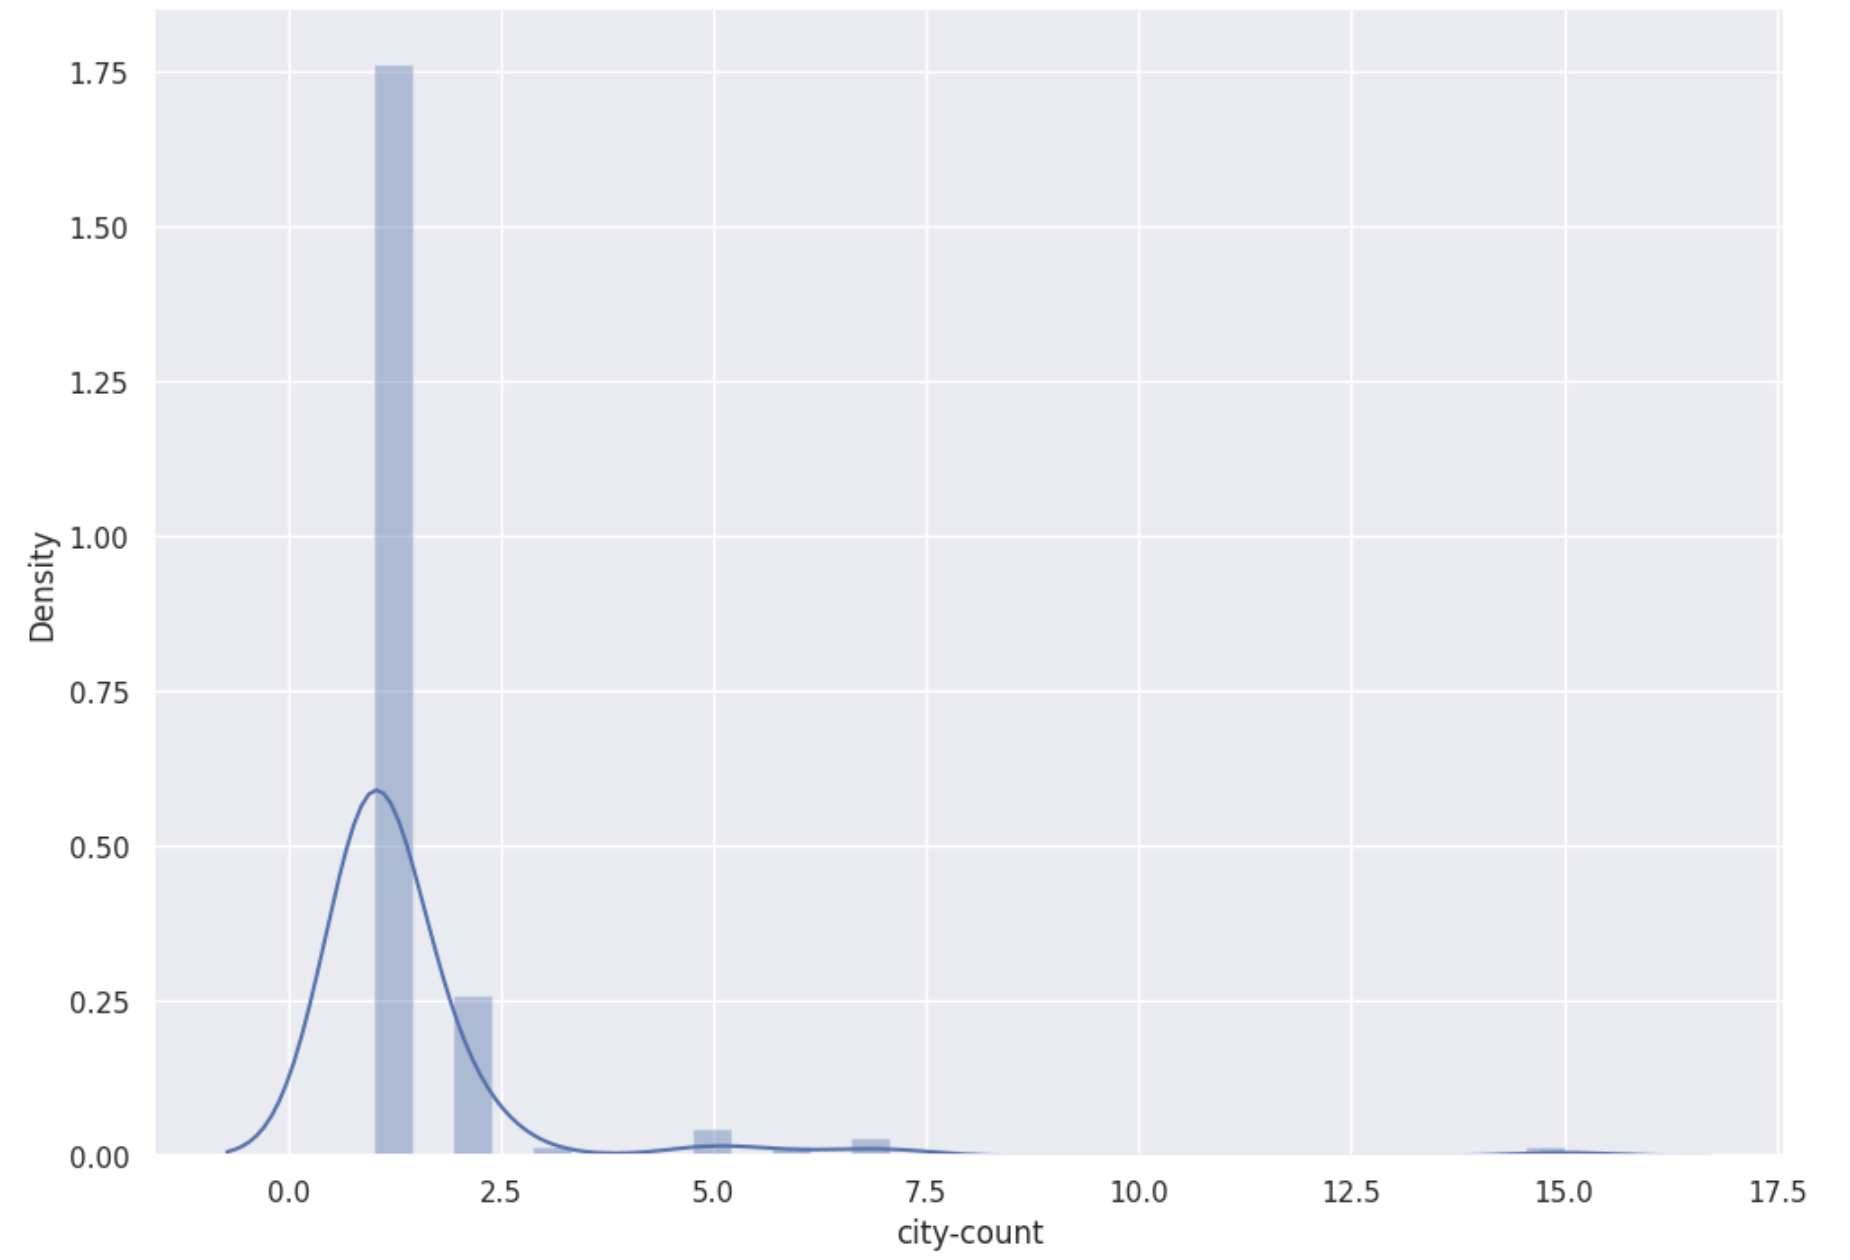
\includegraphics[width=1\textwidth, center]{verteilung_city.png}
    \caption[Verteilung der Städte]{Verteilung der Städte}
    \label{img:verteilung_city}
\end{figure}

Die Analyse der Abbildung \ref{img:verteilung_city} offenbart, dass die überwiegende Mehrheit der in der Datenbank erfassten Städte lediglich über ein einziges Hotel verfügt, welches happyhotel in Anspruch nimmt. Zugleich verdeutlicht die Abbildung \ref{img:verteilung_city}, dass es lediglich einen geringen Anteil von Städten gibt, in denen fünf oder mehr Hotels registriert sind. Dies ist etwas problematisch, da das Feature \emph{City} zu unausgewogen ist und so nicht mit in das Modell gegeben werden kann. Es muss also in einer anderen Form verwendet werden.
\newline
\newline
Momentan werden, wie in der Abbildung \ref{img:all_Features_2} gezeigt, die Stadt und die Region als zwei separate Features aufgelistet. Die Idee ist es nun die zwei Features zu verschmelzen und die Hotels in Regionen aufzuteilen um mehr Informationen zu erhalten. Anstatt also Region und Stadt separat zu haben soll es ein Feature Region geben, welches wie folgt aufgebaut ist: 

\begin{itemize}
    \item Befindet sich innerhalb einer Stadt Fünf oder mehr Hotels, so wird die Stadt ohne jegliche Modifikation als Region genommen.
    \item Befindet sich innerhalb einer Stadt weniger als Fünf Hotels, so setzt sich die Region aus der ursprünglichen Region, also dem Bundesland und der Größe der Stadt zusammen nach dem Schema: {Region}-{Größe}
\end{itemize}

Für die Idee muss zunächst ermittelt werden, in welchen Städte sich Fünf oder mehr Hotels befinden. Auch diese Information kann wie folgt Visualisiert werden:

\begin{figure}[h]
    \centering
    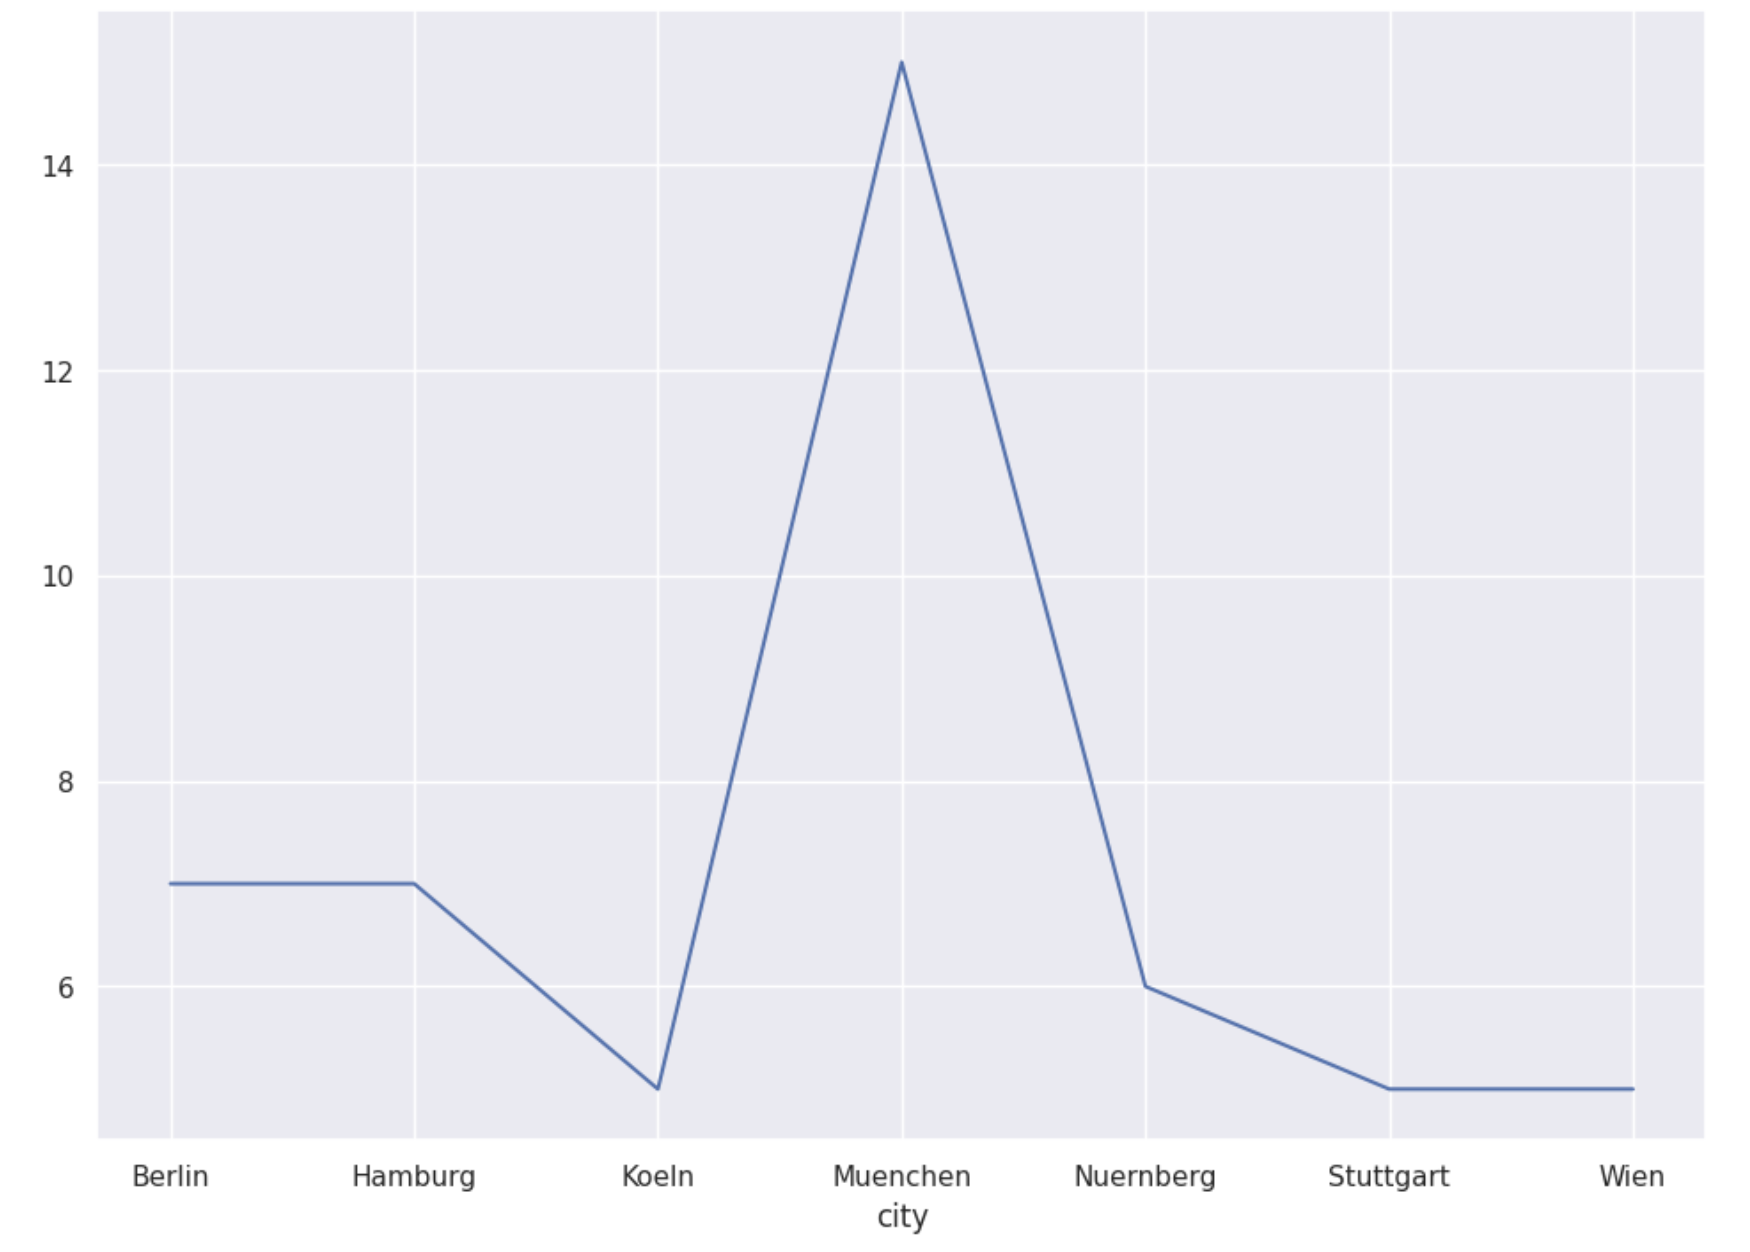
\includegraphics[width=1\textwidth, center]{city_five_or_more.png}
    \caption[Städte mit Fünf oder mehr Hotels]{Städte mit Fünf oder mehr Hotels}
    \label{img:city_five_or_more}
\end{figure}

Ganz klar zu erkennen ist, dass die Sieben Städte Berlin, Hamburg, Köln, München, Nürnberg, Stuttgart, und Wien die Städte sind, in denen Fünf oder mehr Hotels vorhanden sind. Die aufgelisteten Städte können dementsprechend so übernommen werden und für alle anderen wird die Regel von oben angewandt.
\newline
Nach der Umformulierung von Region und Stadt sieht der Datensatz wie folgt aus:

\begin{figure}[h]
    \centering
    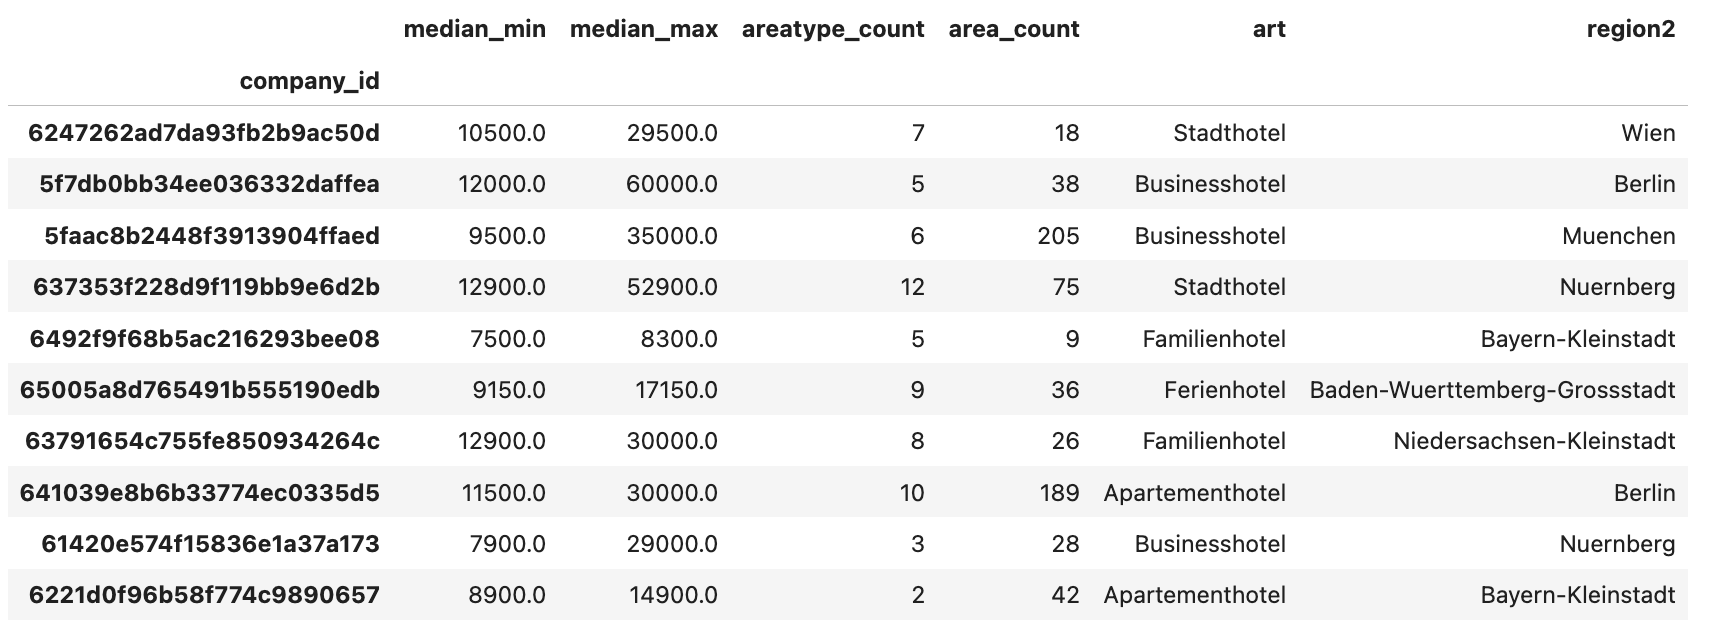
\includegraphics[width=1\textwidth, center]{all_features_3.png}
    \caption[Datensatz nach der Umformulierung]{Datensatz nach der Umformulierung}
    \label{img:all_features_3}
\end{figure}

Auch hier soll wieder die Verteilung visualisiert werden

\begin{figure}[h]
    \centering
    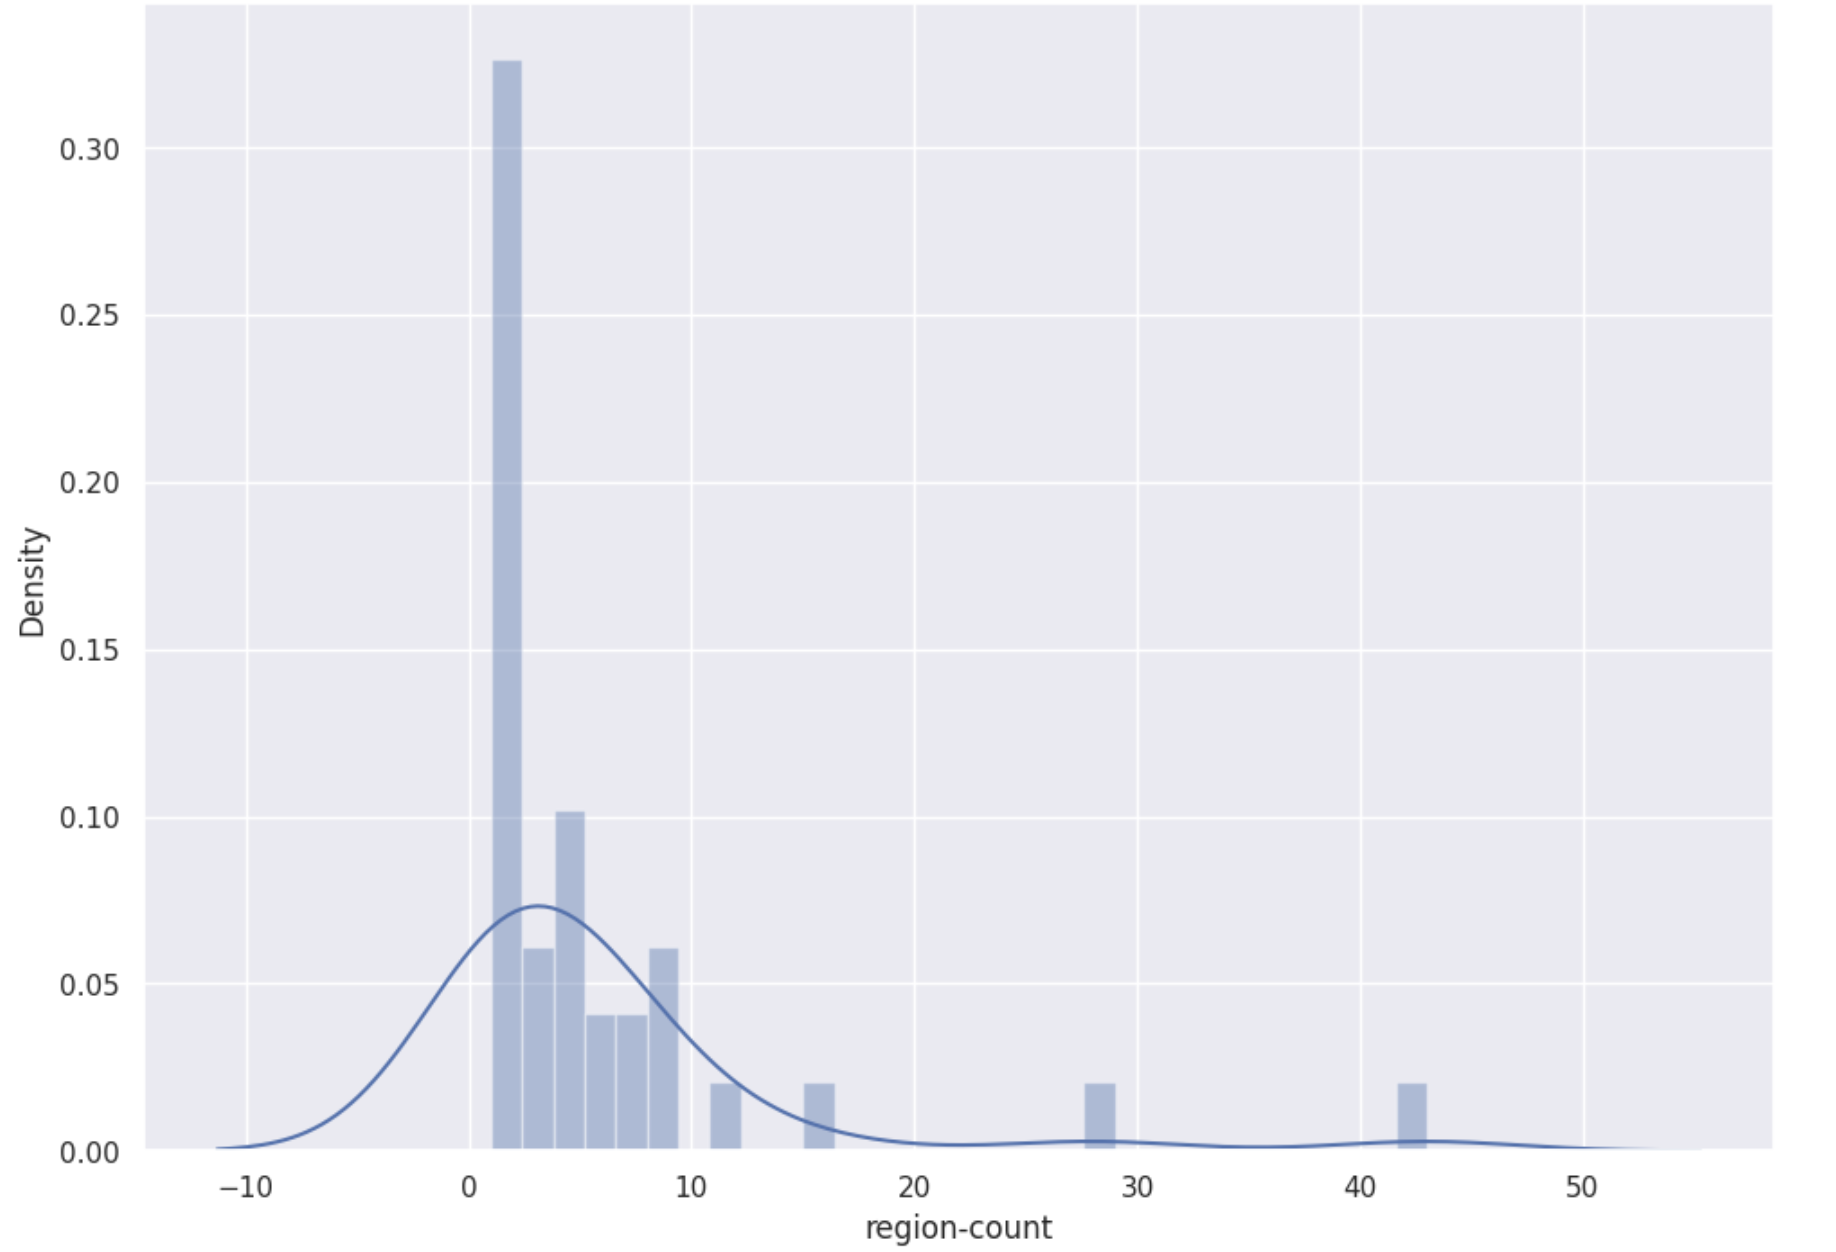
\includegraphics[width=1\textwidth, center]{verteilung_region2.png}
    \caption[Verteilung des neuen Features \emph{region2}]{Verteilung des neuen Features \emph{region2}}
    \label{img:verteilung_region_2}
\end{figure}

Es zeigt sich, dass noch immer ein großer Anteil des Datensatzes niedrigeren Bereich sich befindet, jedoch konnte mit der Modifikation ein bisschen mehr Varianz in die Daten gebracht werden.

\subsubsection{Preis Features}
Als nächstes sollen die Preis Features, namentlich betitelt mit \emph{median\_min} und \emph{median\_max}, erkundet und visualisiert werden. Hierzu soll wie auch bei der Region zunächst die Verteilung betrachtet werden:
\newpage
\begin{figure}[h]
    \centering
    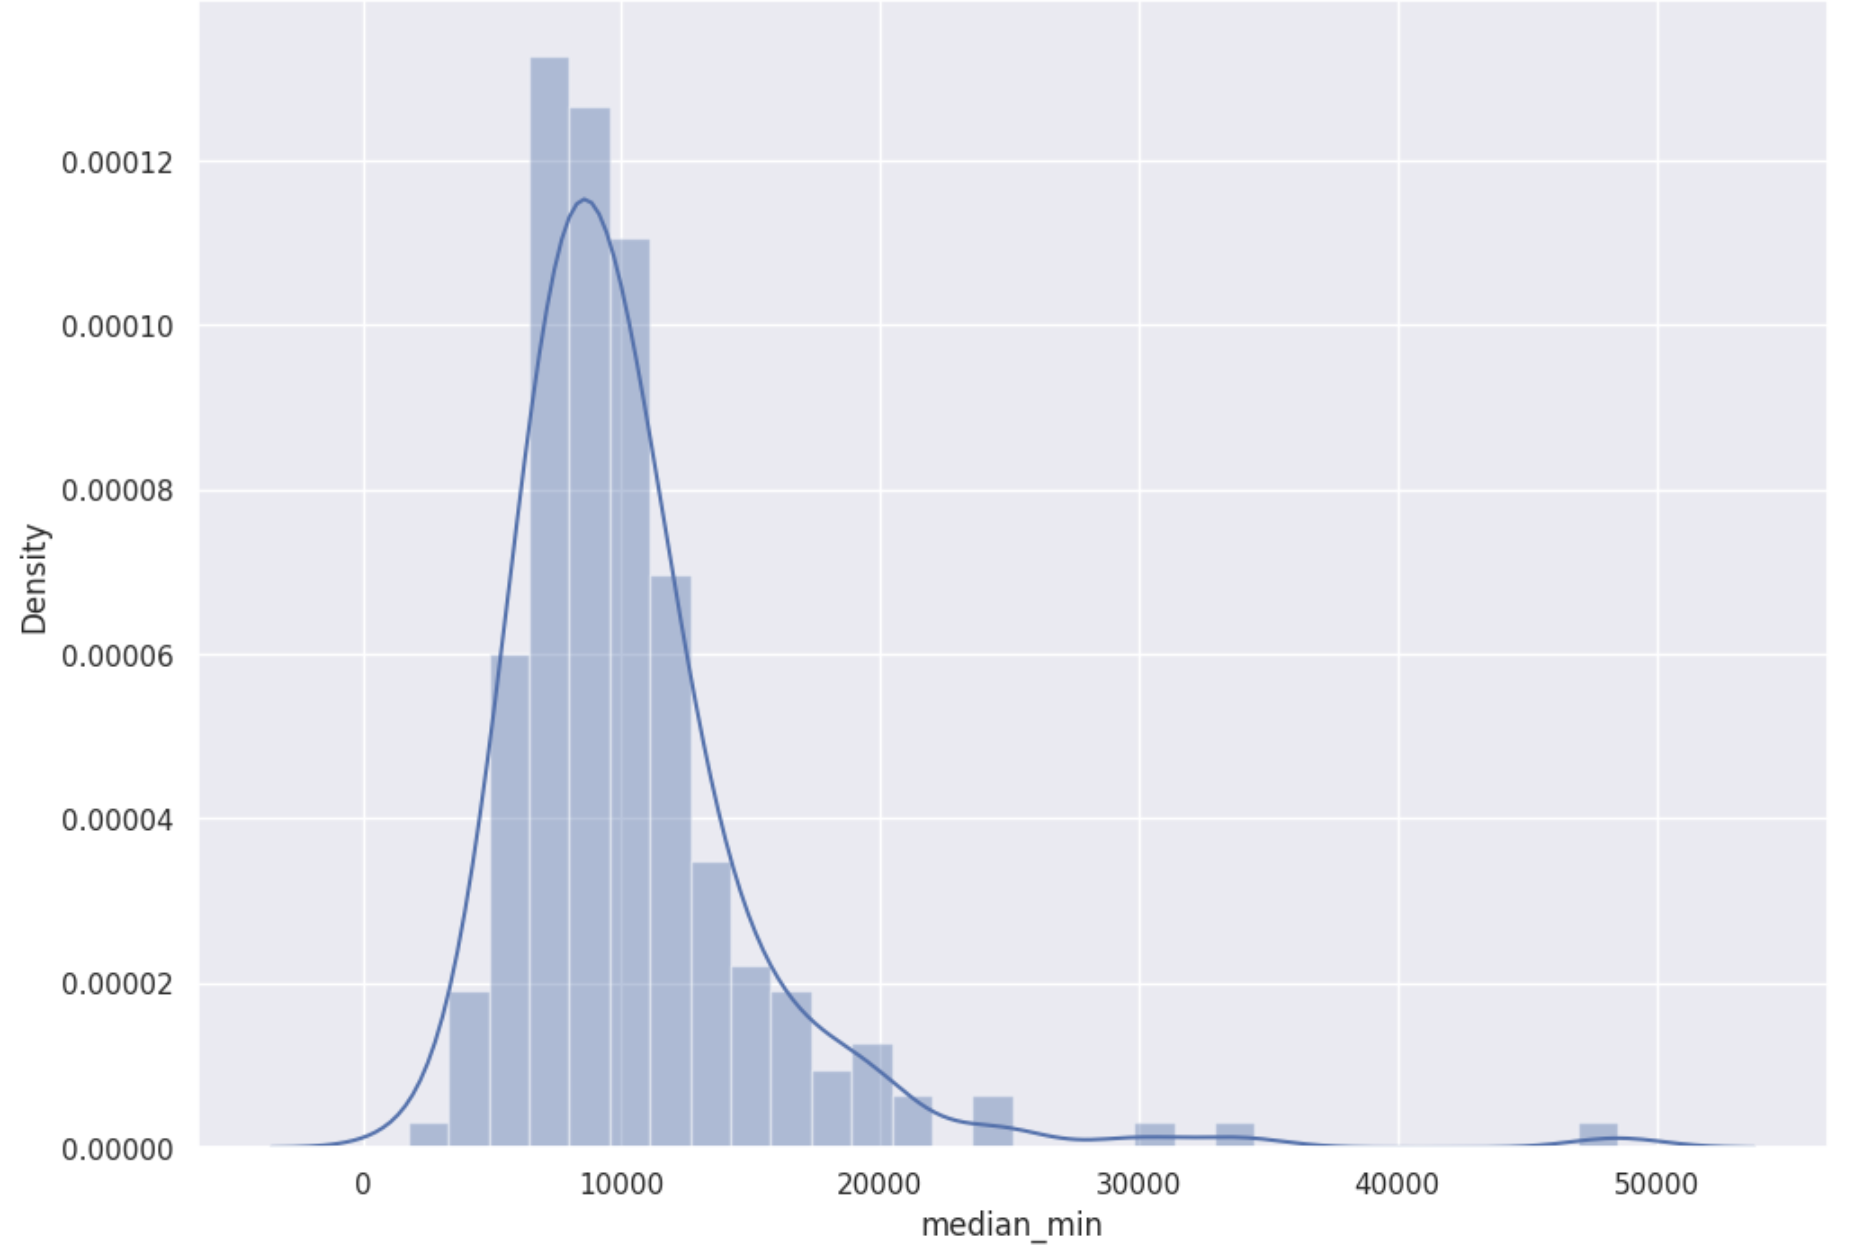
\includegraphics[width=1\textwidth, center]{verteilung_min.png}
    \caption[Verteilung von dem Preis Features \emph{median\_min}]{Verteilung von dem Preis Features \emph{median\_min}}
    \label{img:verteilung_min}
\end{figure}

Abbildung \ref{img:verteilung_min} zeigt, dass das Feature \emph{median\_min} eine Normalverteilung mit ein paar outlier aufweist. Eine Normalverteilung  sagt aus, dass die Verteilung mehr Daten um den Mittelwert herum aufweist. Die Datenverteilung nimmt ab, wenn sich vom Zentrum entfernt wird. Die resultierende Kurve ist symmetrisch zum Mittelwert und bildet eine glockenförmige Verteilung \cite{Shrishty.05.08.2021}.
\newline
\newline
Eine weitere interessante Information die noch aus dem Feature \emph{median\_min} gelesen werden kann, ist der Durchschnittliche Wert Region. Dazu soll der Datensatz nach der Region gruppiert werden und den Durchschnittlichen Wert ermittelt werden.
\newpage
\begin{figure}[h]
    \centering
    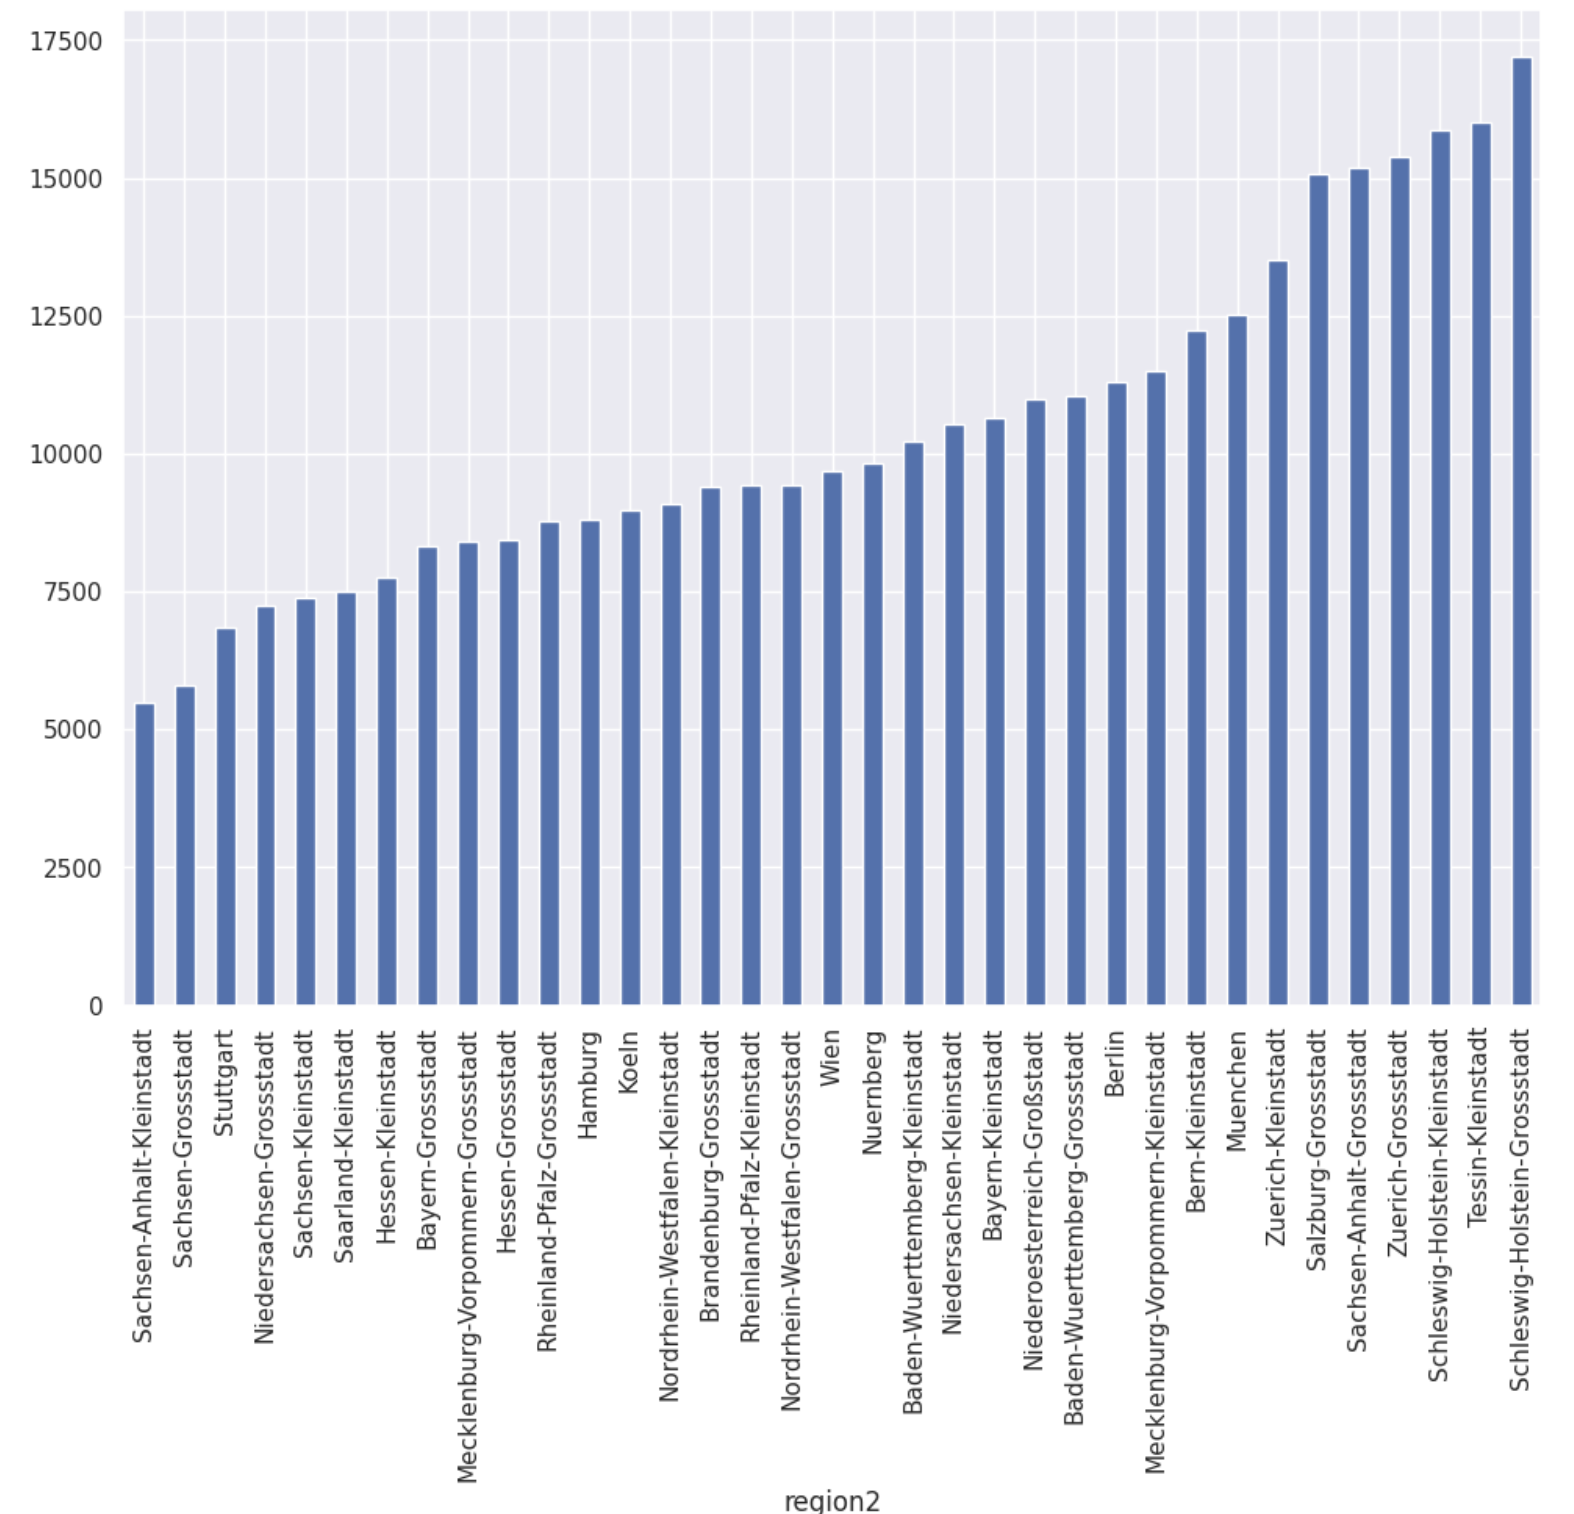
\includegraphics[width=0.6\textwidth, center]{avg_min_city.png}
    \caption[Durchschnittlicher minimal Preis pro Region]{Durchschnittlicher minimal Preis pro Region}
    \label{img:avg_min_city}
\end{figure}

Die Erkenntnis die aus der Abbildung \ref{img:avg_min_city} genommen werden kann, ist die, dass es einen deutlichen unterschied macht, in welcher Region das Hotel liegt wenn auf den Minimalen Median Preis des Hotel geschaut wird. Das gleich kann auch mit dem Maximalen Median Preis eines Hotels gemacht werden. Auch hier soll sich zunächst die Verteilung visualisiert werden:

\begin{figure}[h]
    \centering
    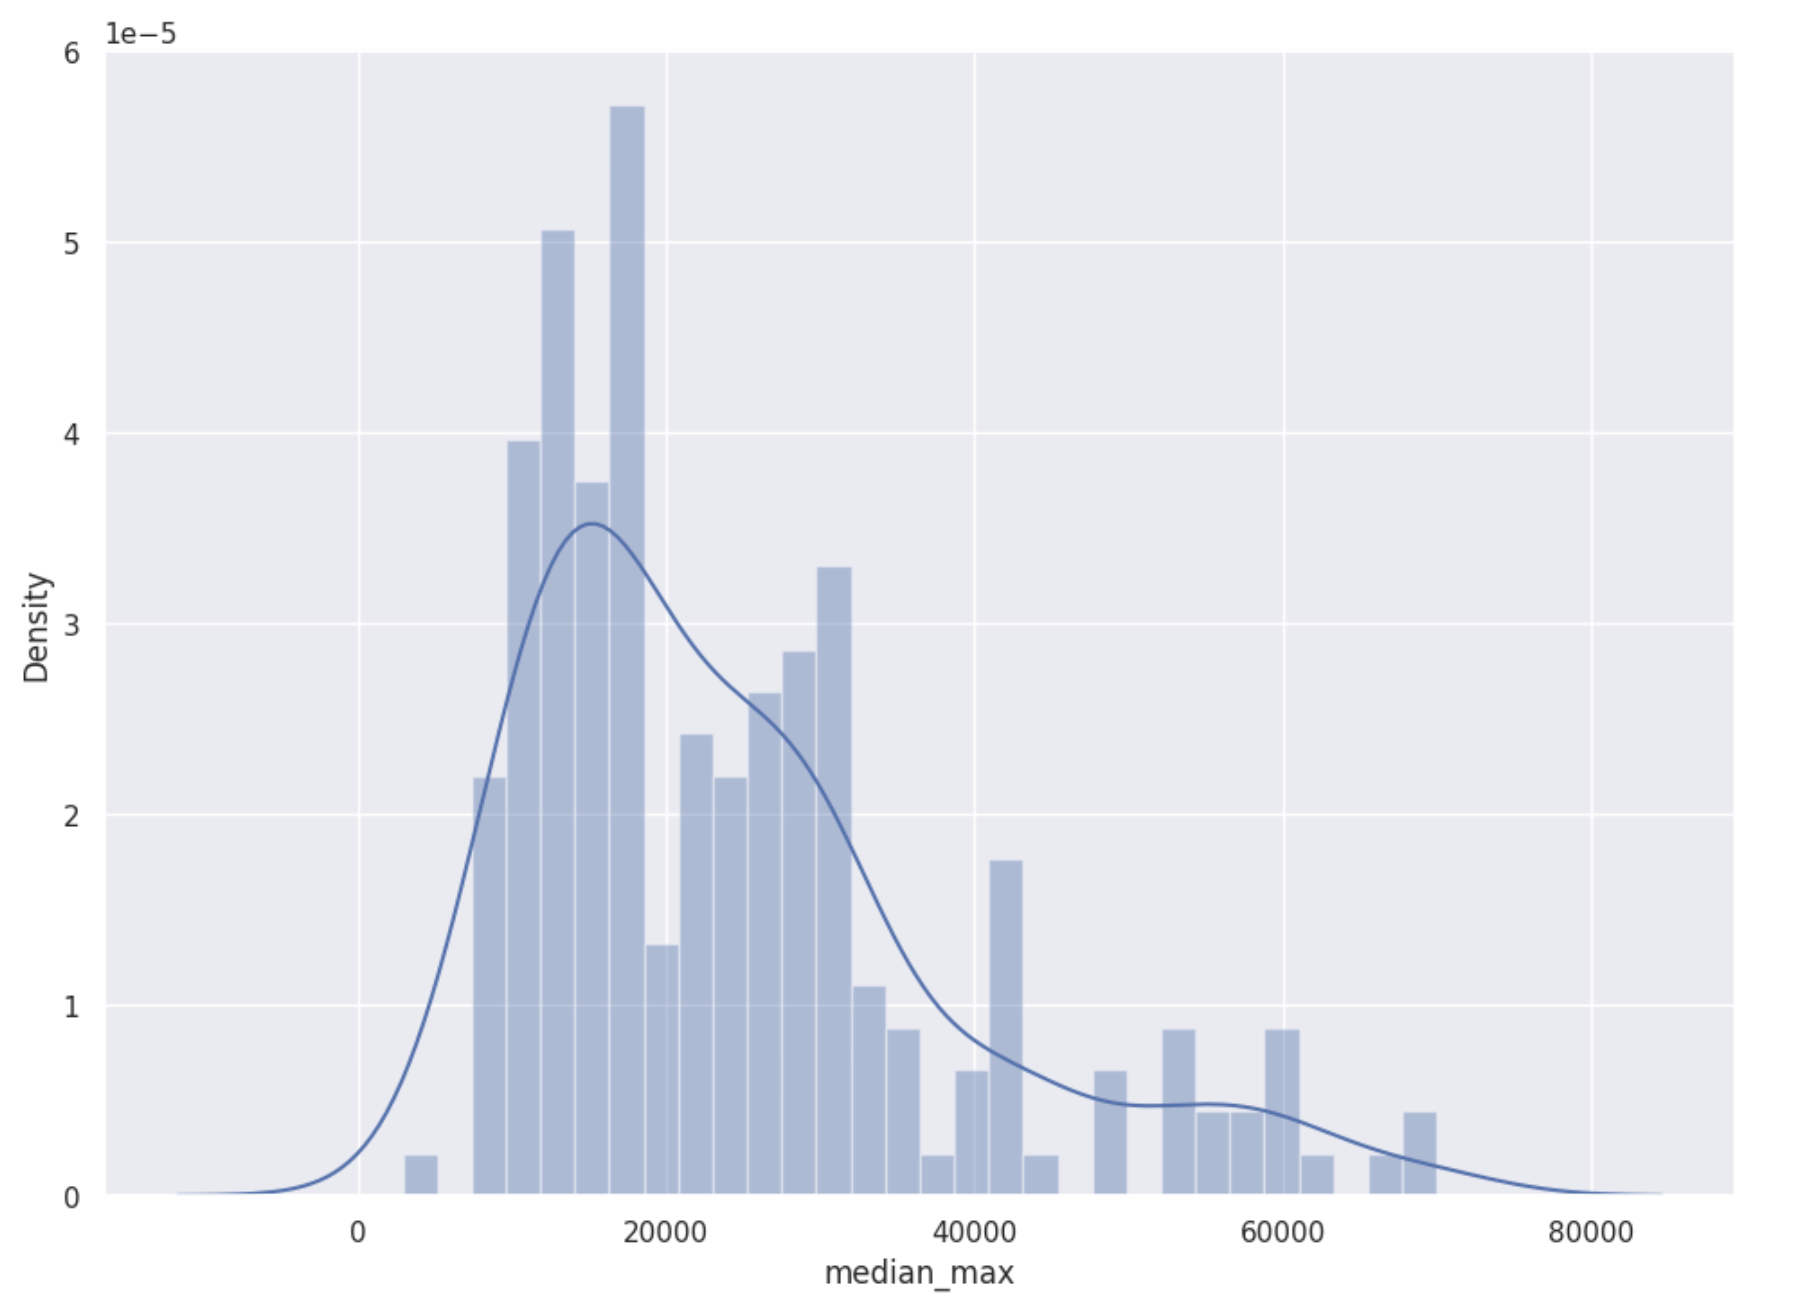
\includegraphics[width=0.6\textwidth, center]{verteilung_max.png}
    \caption[Verteilung von dem Preis Features \emph{median\_max}]{Verteilung von dem Preis Features \emph{median\_max}}
    \label{img:verteilung_max}
\end{figure}

Anders als bei dem Minimalen Median Preis, kann bei dem Maximalen Median Preis keine Normalverteilung erkannt werden. Hier wirken die Werte recht verstreut.

\begin{figure}[h]
    \centering
    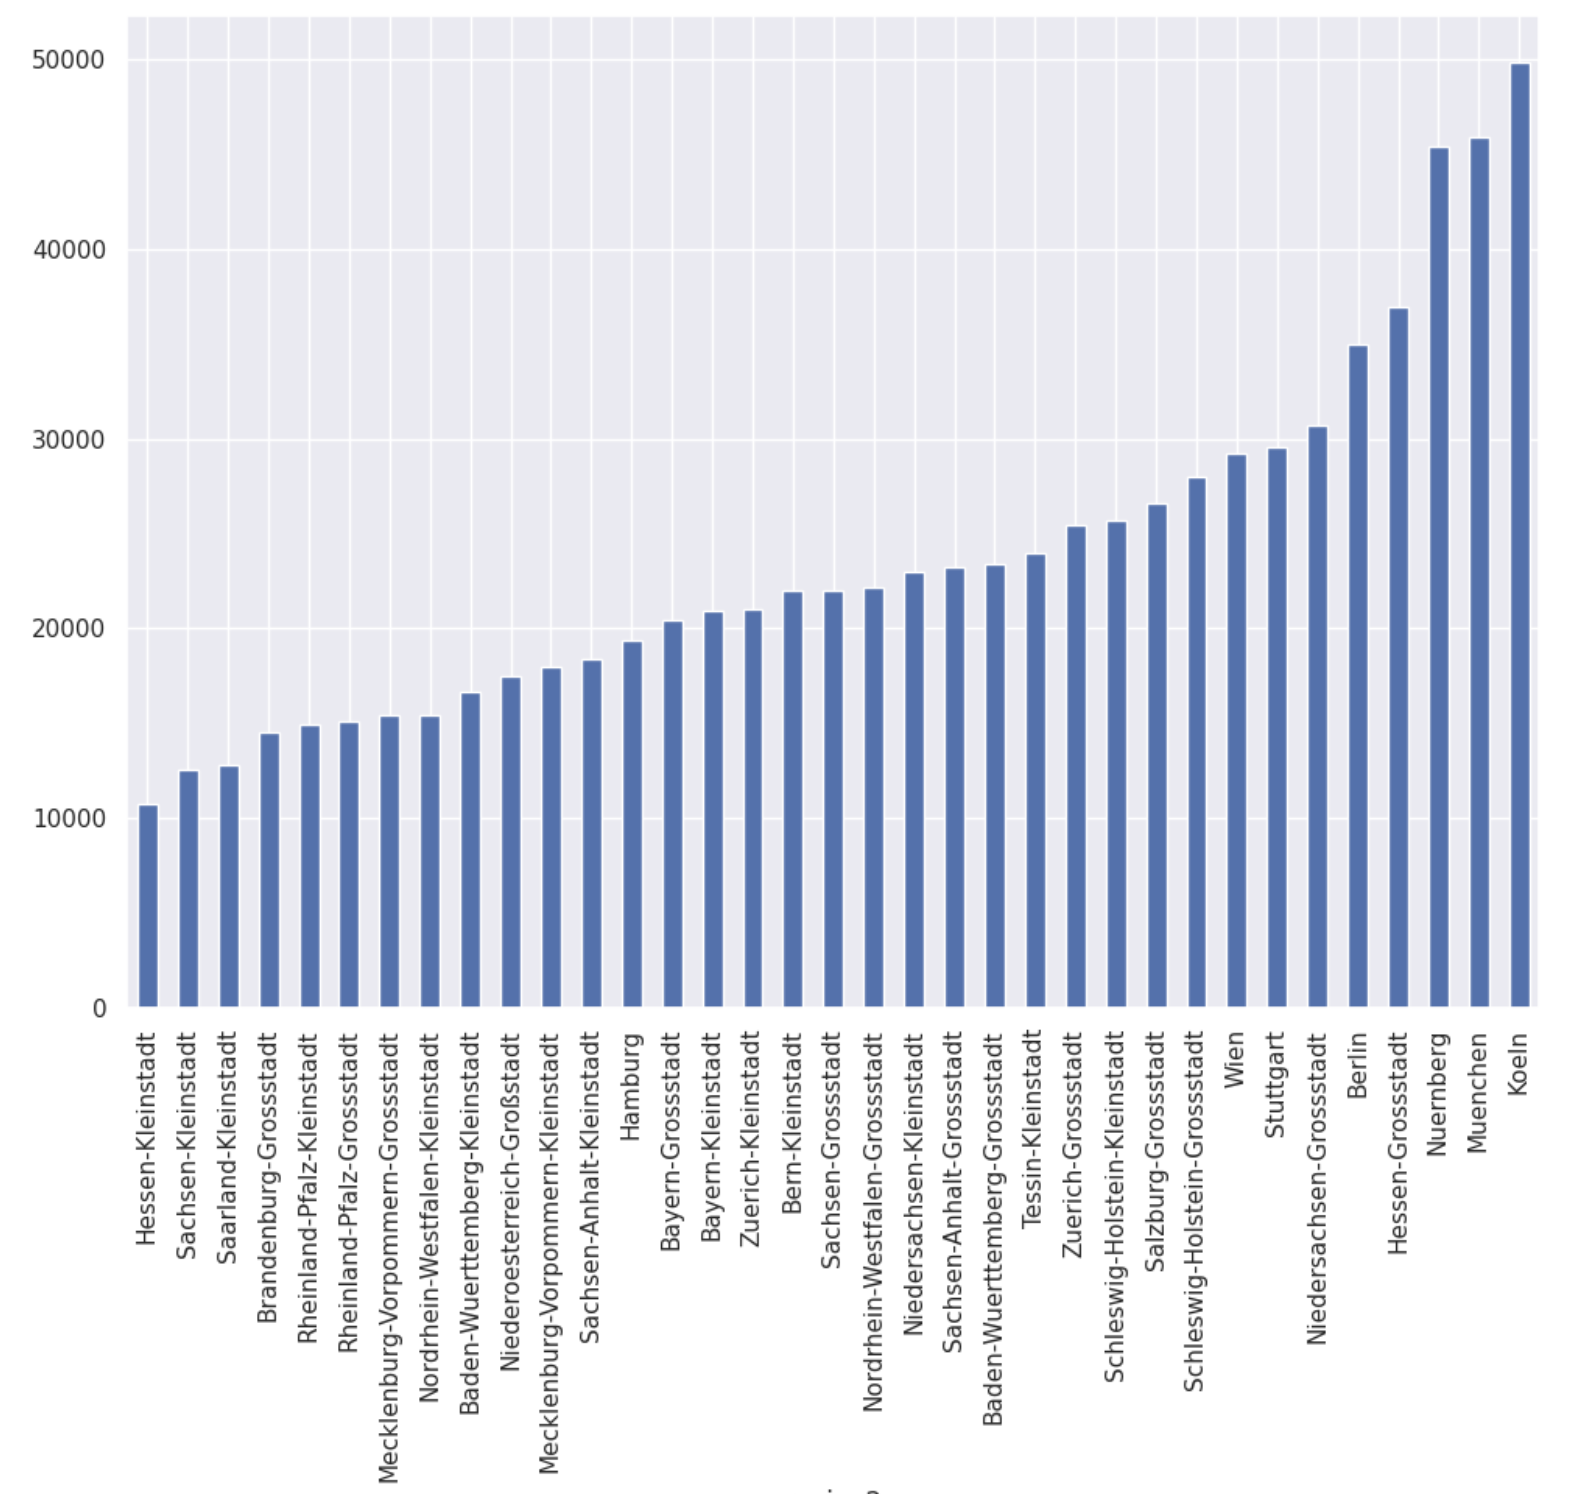
\includegraphics[width=1\textwidth, center]{avg_max_region.png}
    \caption[Durchschnittlicher maximal Preis pro Region]{Durchschnittlicher maximal Preis pro Region}
    \label{img:avg_max_city}
\end{figure}

Abbildung \ref{img:avg_max_city} zeigt, dass es auch deutliche Unterschiede bei den einzelnen Regionen gibt. Eine weitere interessante Erkenntnis ist die, dass es bei dem Maximalen Median Preis eher so ist, dass die Großstädte wie Köln und München eher zu einem höheren Maximalen Preis tendieren.

\subsubsection{Hotelart Feature}
Die Hotelart bildet einen essenziellen Bestandteil, um umfassende Einblicke in die Charakteristiken eines Hotels zu gewinnen. Sie liefert nicht nur Informationen über den Zweck und die Ausrichtung der Unterkunft, sondern ermöglicht auch eine präzise Identifikation der Zielgruppe, die das Hotel anspricht \cite{User.20.01.2024}. Die Zielgruppe eines Hotels ist zudem eine wertvolle Information wenn es darum geht Preise für das Hotel zu gestalten, zumindest ist so die Annahme. Auch in diesem Fall kann wieder nach der Hotelart gruppiert werden und jeweils der Minimale und Maximale durchschnittliche Preis angezeigt werden.

\begin{figure}[h]
    \centering
    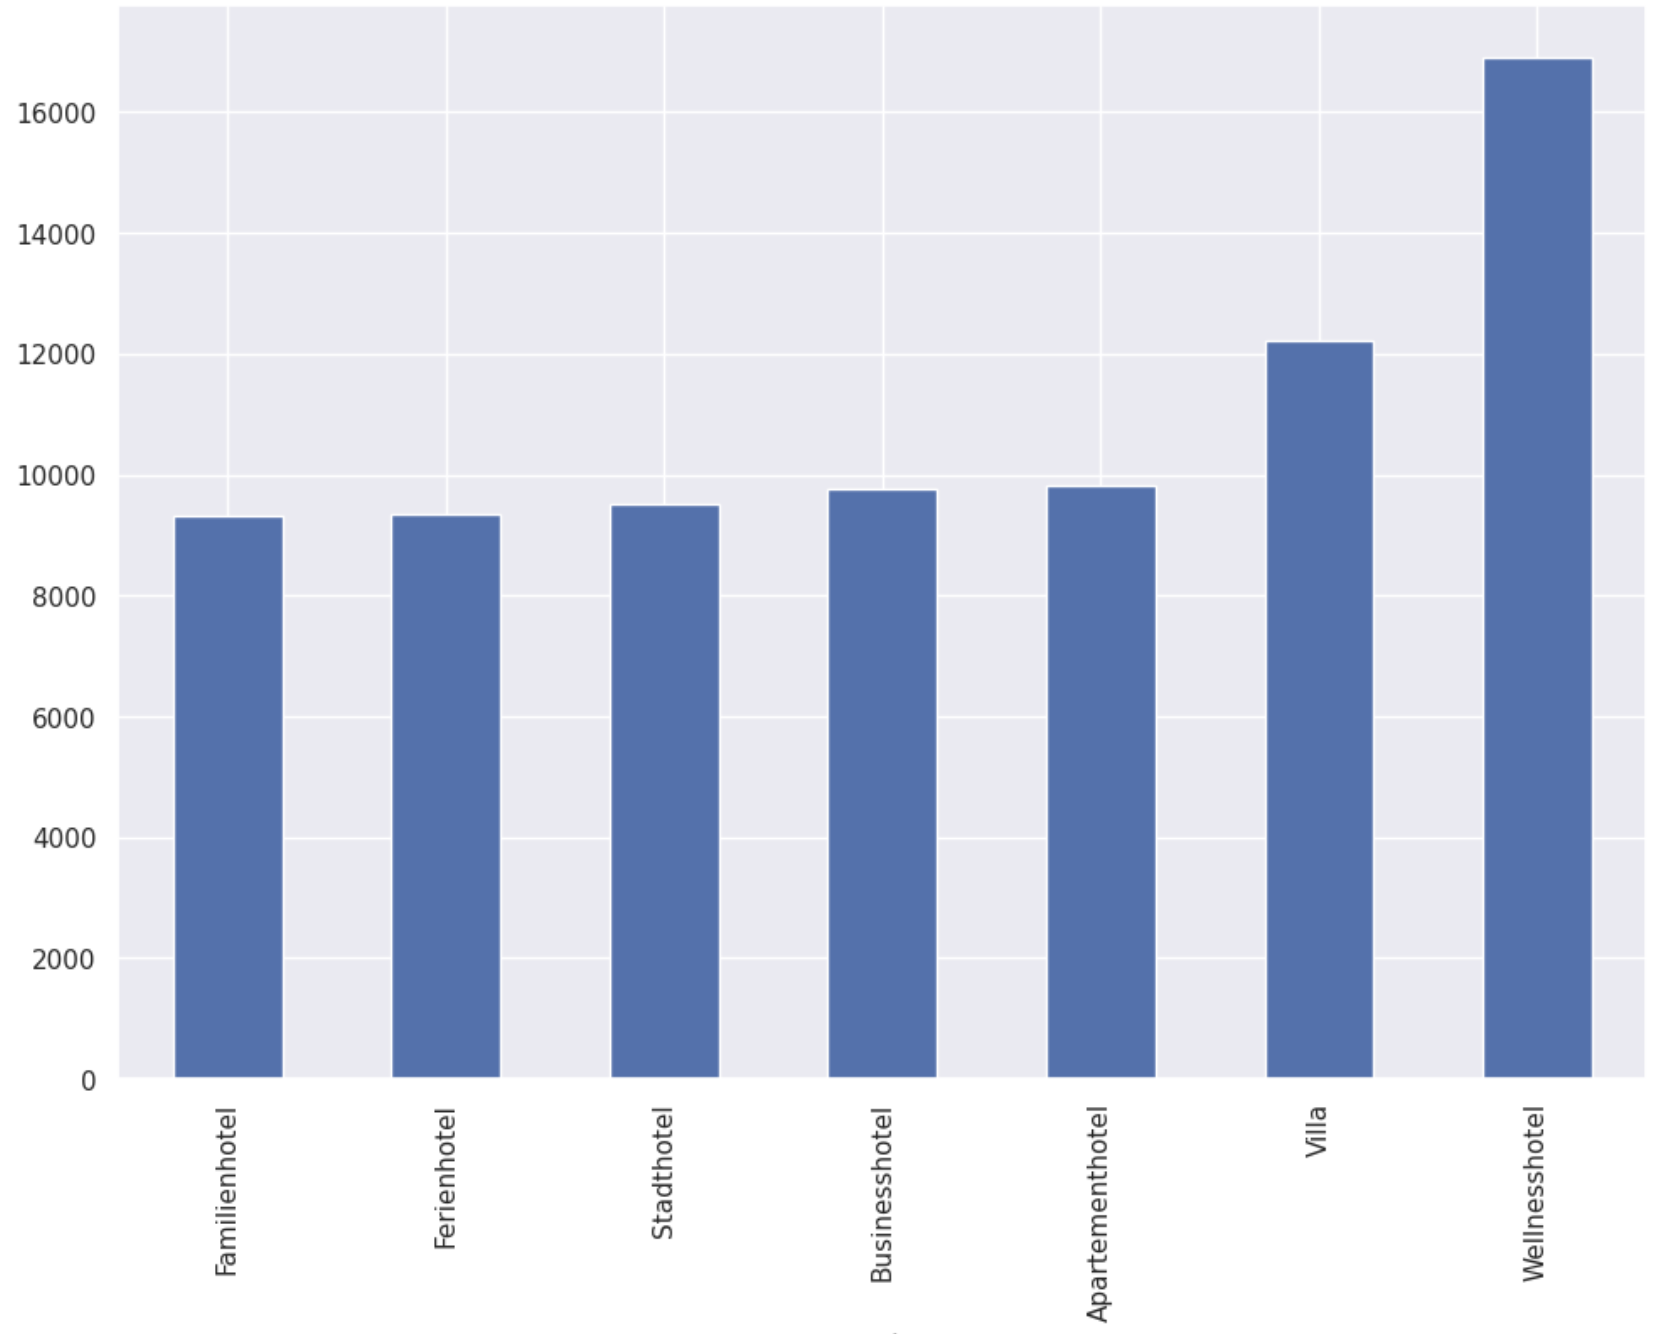
\includegraphics[width=0.6\textwidth, center]{avg_min_art.png}
    \caption[Durchschnittlicher minimal Preis pro Hotelart]{Durchschnittlicher minimal Preis pro Hotelart}
    \label{img:avg_min_art}
\end{figure}

\begin{figure}[h]
    \centering
    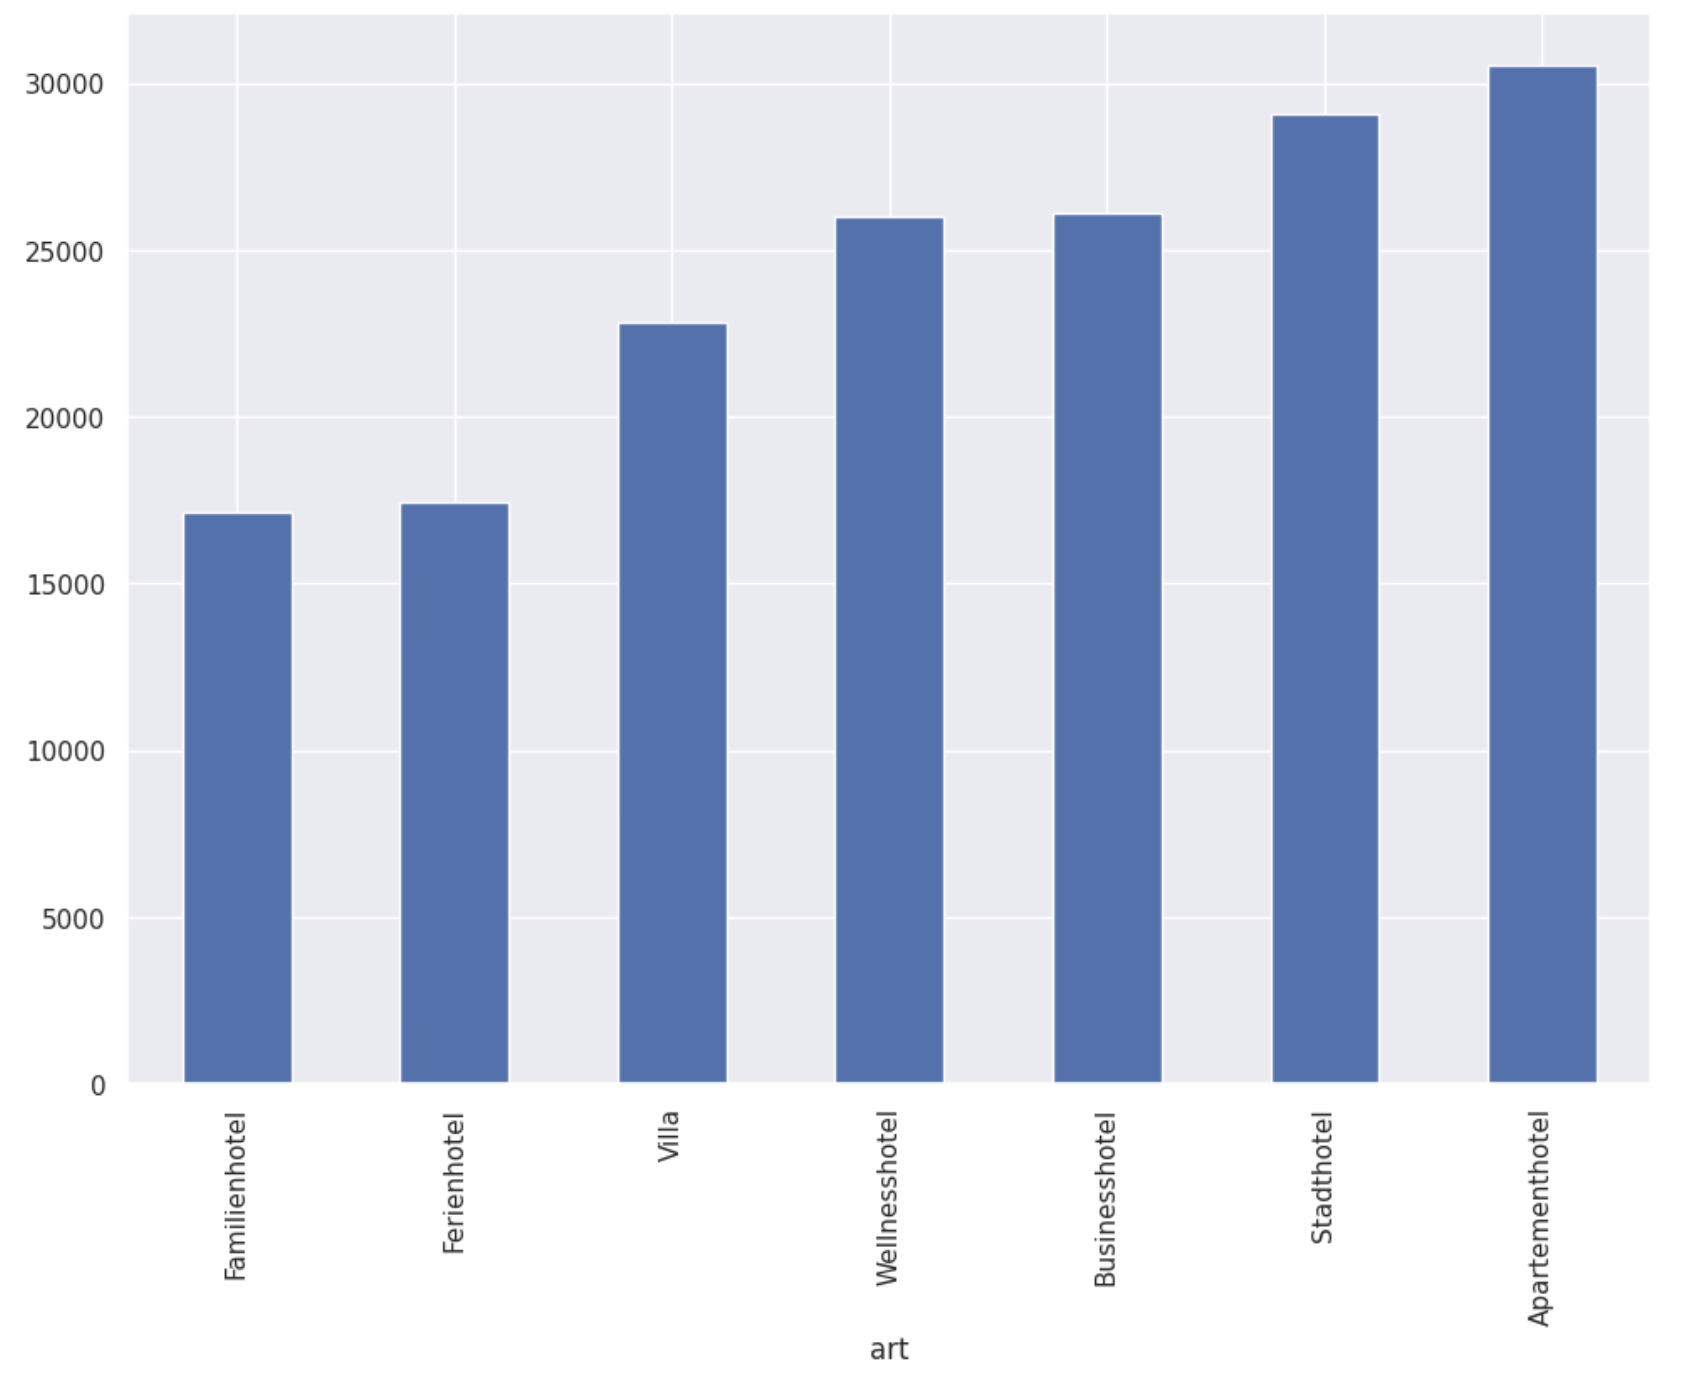
\includegraphics[width=0.6\textwidth, center]{avg_max_art.png}
    \caption[Durchschnittlicher maximal Preis pro Hotelart]{Durchschnittlicher maximal Preis pro Hotelart}
    \label{img:avg_max_art}
\end{figure}

Anhand von den zwei Abbildungen \ref{img:avg_min_art} und \ref{img:avg_max_art} zeigt sich, dass tatsächlich einen unterschied bei den Preisen auf die Hotelart bezogen gibt. Zudem zeigt sich, dass die zwei Hotelarten \emph{Ferienhotel} und \emph{Familienhotel} in beiden Fällen die gleiche Information wiedergibt und somit auch zu \emph{Ferienhotel} zusammengefasst werden kann. Zudem könnten anhand von \emph{median\_min} noch weitere Hotelarten zusammengefasst werden, jedoch wenn beide Informationen zusammen betrachtet werden, so bleibt es lediglich bei \emph{Ferienhotel} und \emph{Familienhotel}.

\subsubsection{Zimmer Features}
Die letzten zwei Features innerhalb des Datensatzes sind die Features \emph{area\_count} und \emph{areatype\_count} welche die Größe des jeweiligen Hotels repräsentieren. Die Frage die sich hier also stellt ist, ob das Preisverhältnis in irgendeiner Art mit der Größe des Hotels zusammenhängen kann. Hierzu soll zunächst auch erstmal die Verteilung der Zimmeranzahl angeschaut werden:

\begin{figure}[h]
    \centering
    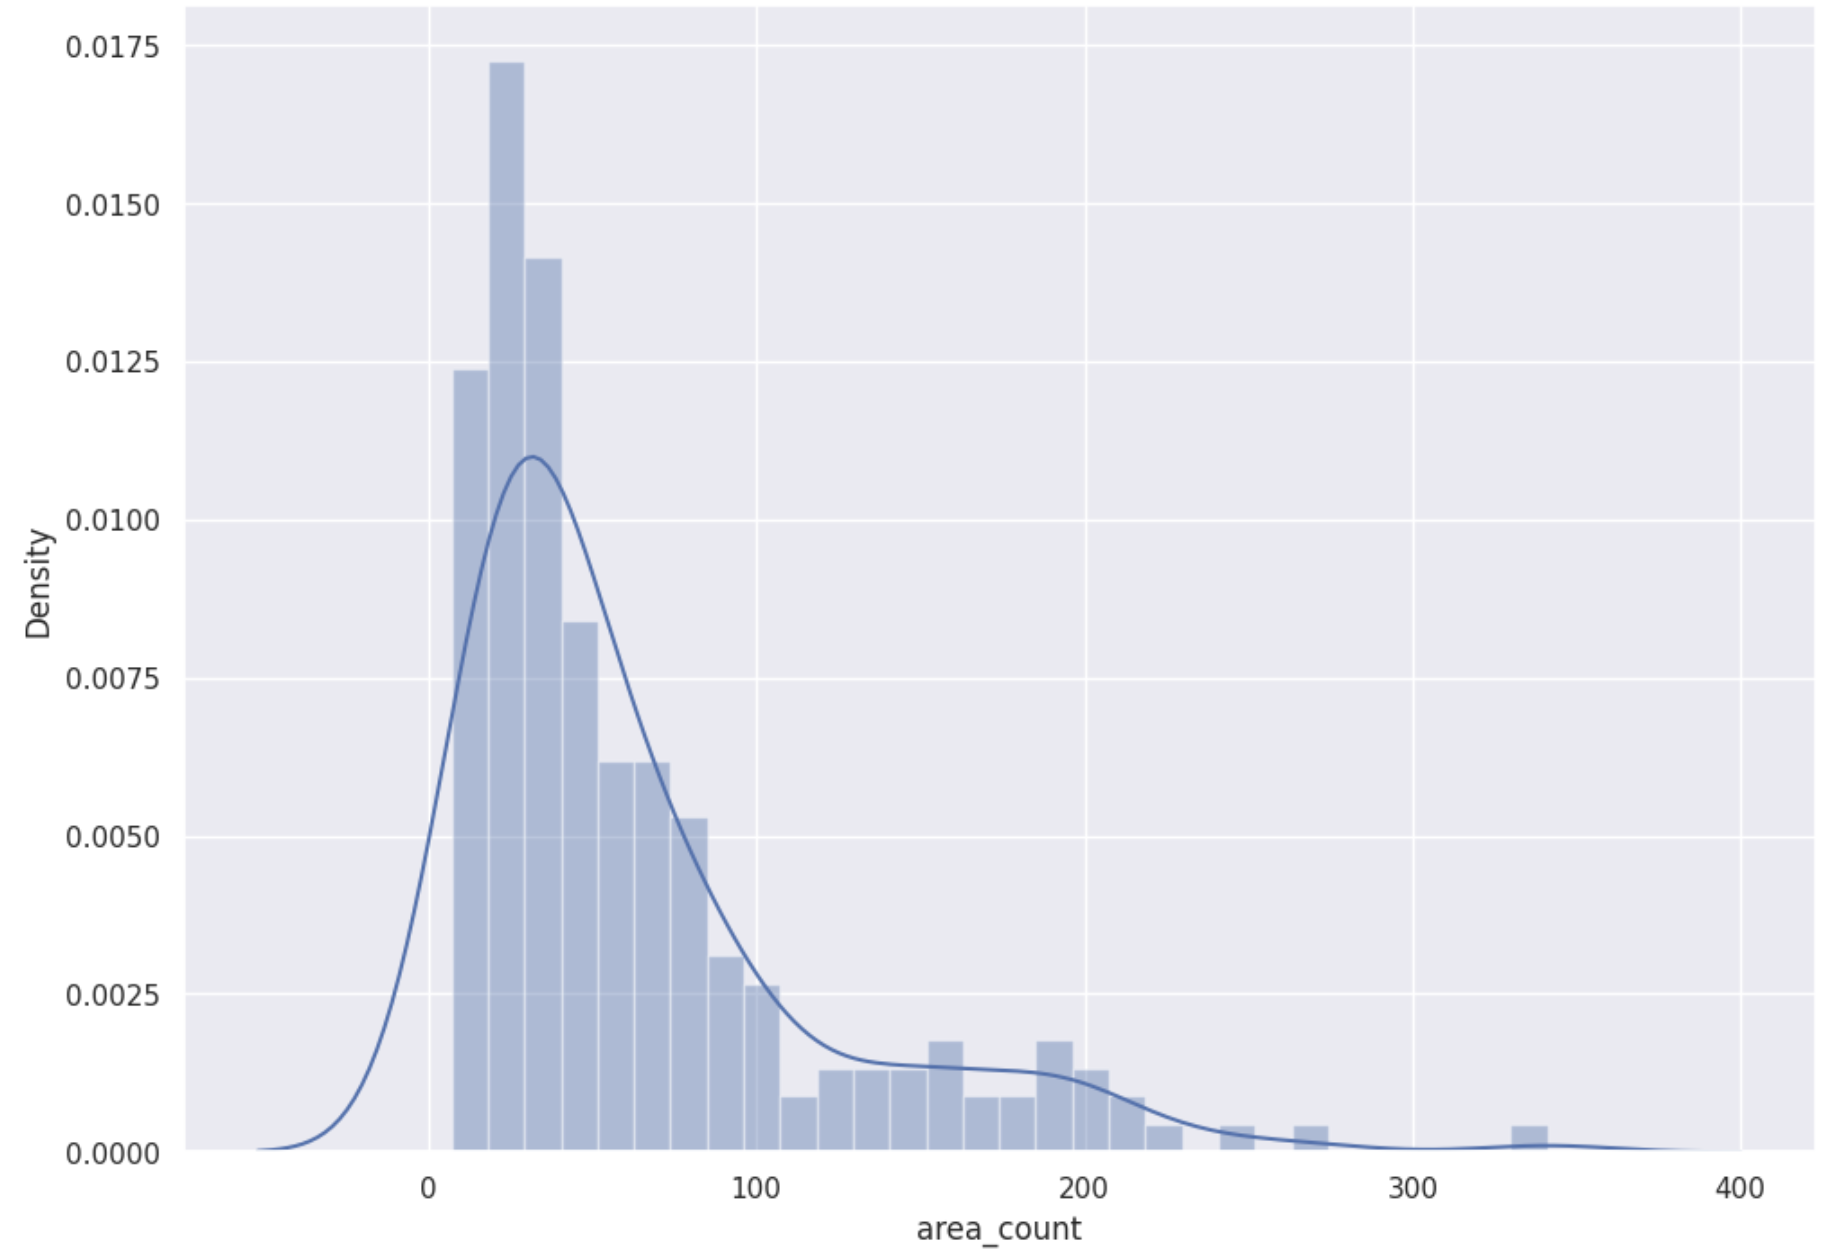
\includegraphics[width=0.6\textwidth, center]{verteilung_area_count.png}
    \caption[Verteilung nach Zimmeranzahl]{Verteilung nach Zimmeranzahl}
    \label{img:verteilung_area_count}
\end{figure}

Die Verteilung zeigt, dass auch recht ausgeprägt ist und nur im Ansatz einer Normalverteilung gleicht. Des Weiteren soll nach der Anzahl der Zimmer gruppiert werden um zu überprüfen wie oft jeder Anzahl vorkommt:

\begin{figure}[h]
    \centering
    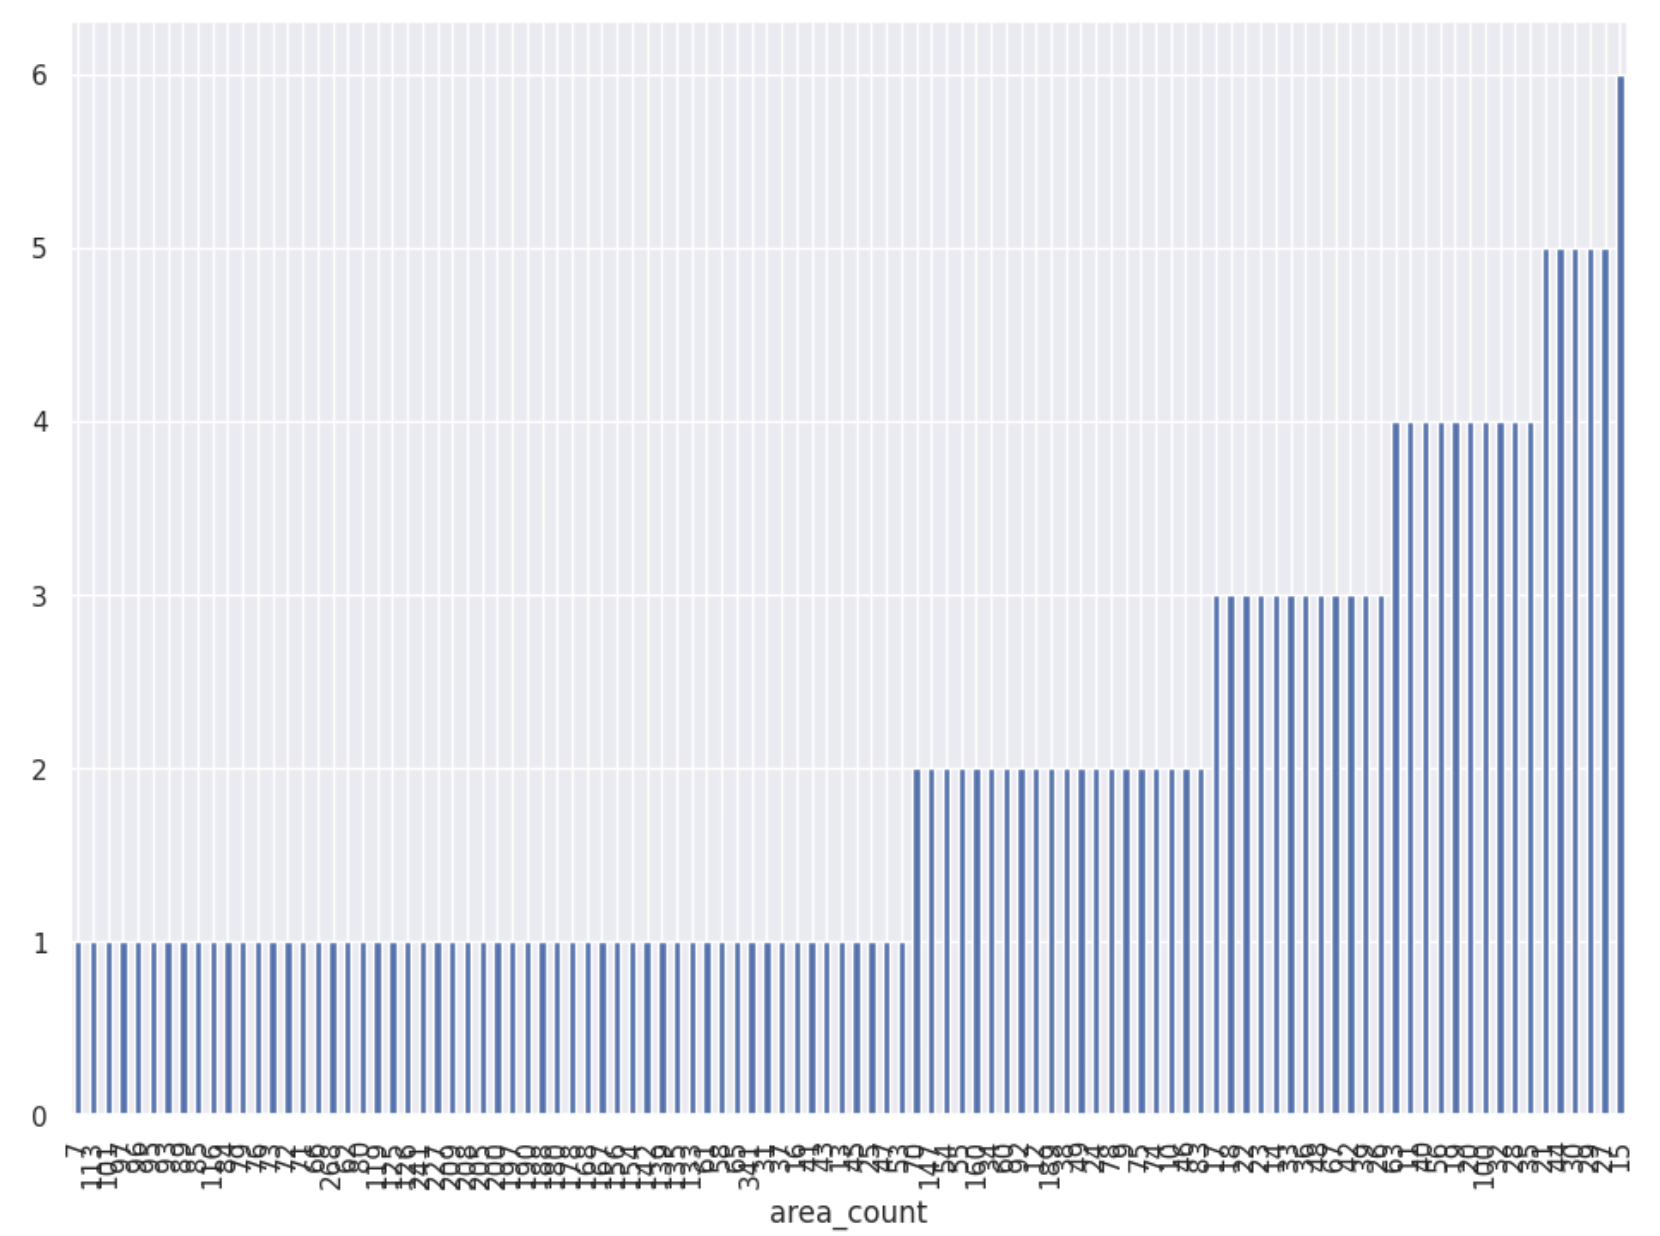
\includegraphics[width=0.6\textwidth, center]{group_area_count.png}
    \caption[Häufigkeit der Zimmeranzahl im Datensatz]{Häufigkeit der Zimmeranzahl im Datensatz}
    \label{img:haufigkeit_area_count}
\end{figure}
Abbildung \ref{img:haufigkeit_area_count} hat gezeigt, dass das Feature \emph{area\_count} zu ausgeprägt ist. Aufgrund dessen, dass das Feature zu ausgeprägt ist und keine Idee vorhanden ist, wie dieses Feature umformuliert werden könnte, wurde beschlossen \emph{area\_count} und \emph{areatype\_count} aus dem Datensatz zu entfernen.
\newline
\newline
Der finale Datensatz welcher für das Modell benutzt werden soll, sieht wie folgt aus:

\begin{figure}[h]
    \centering
    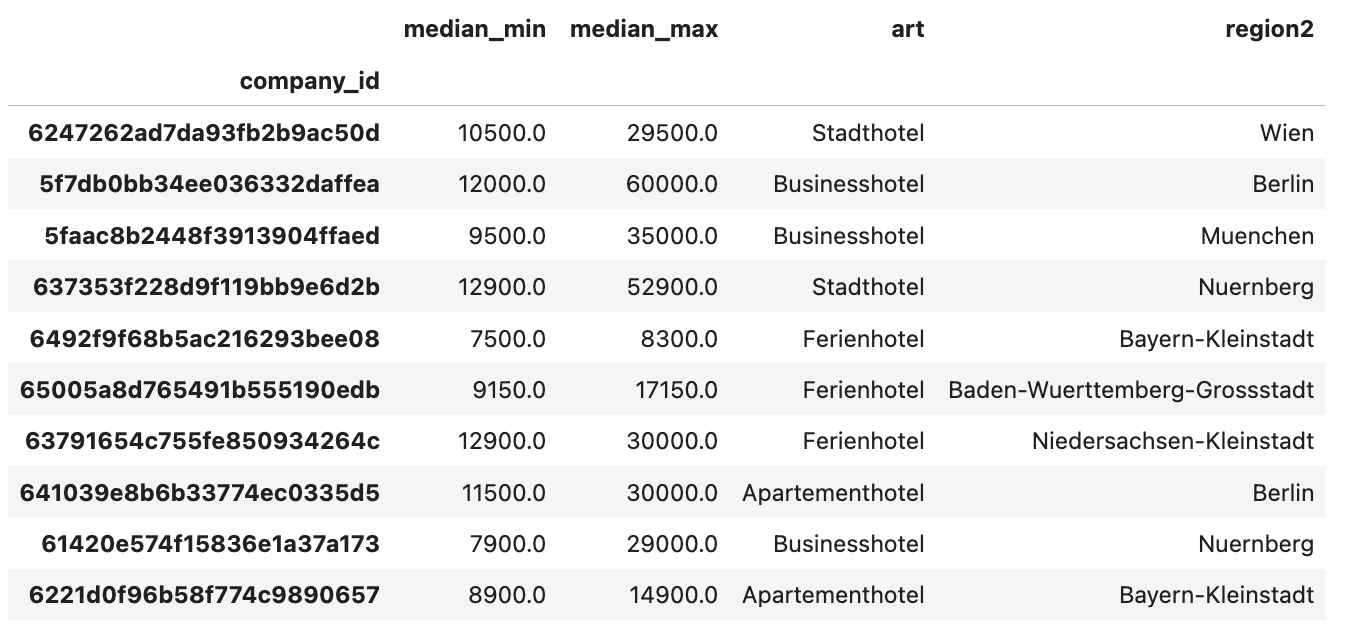
\includegraphics[width=1\textwidth, center]{all_features_4.png}
    \caption[Finaler Datensatz für das Modell]{Finaler Datensatz für das Modell}
    \label{img:all_features_4}
\end{figure}
\subsection{Evaluation der Ähnlichen Hotels}
\label{subsec:Evaluation_1}
Der vorliegende Datensatz ist nun verfügbar, und grundsätzlich kann die Modellierung fortgesetzt werden. Allerdings stellt sich die Frage, ob die identifizierten Hotels tatsächlich ähnlich zum ursprünglichen Hotel sind. Es ist von entscheidender Bedeutung, nachzuweisen, dass die ausgewählten Hotels auf irgendeine Weise miteinander vergleichbar sind. Aus diesem Grund wird im nachfolgenden Abschnitt ein Mechanismus entwickelt, um die Ähnlichkeit der Hotels zu überprüfen und zu gewährleisten.
\newline
\newline
Angesichts des angestrebten Ziels, nämlich der dynamischen Generierung von Preisen, wurde zunächst in Erwägung gezogen, die Preise der einzelnen Hotels zu vergleichen. Zu diesem Zweck wurde initial ein \emph{Dataframe} erstellt, das sämtliche gültigen Hotels sowie ihre Preisinformationen für einen bestimmten Zeitraum umfasst.
\newpage
\begin{figure}[h]
    \centering
    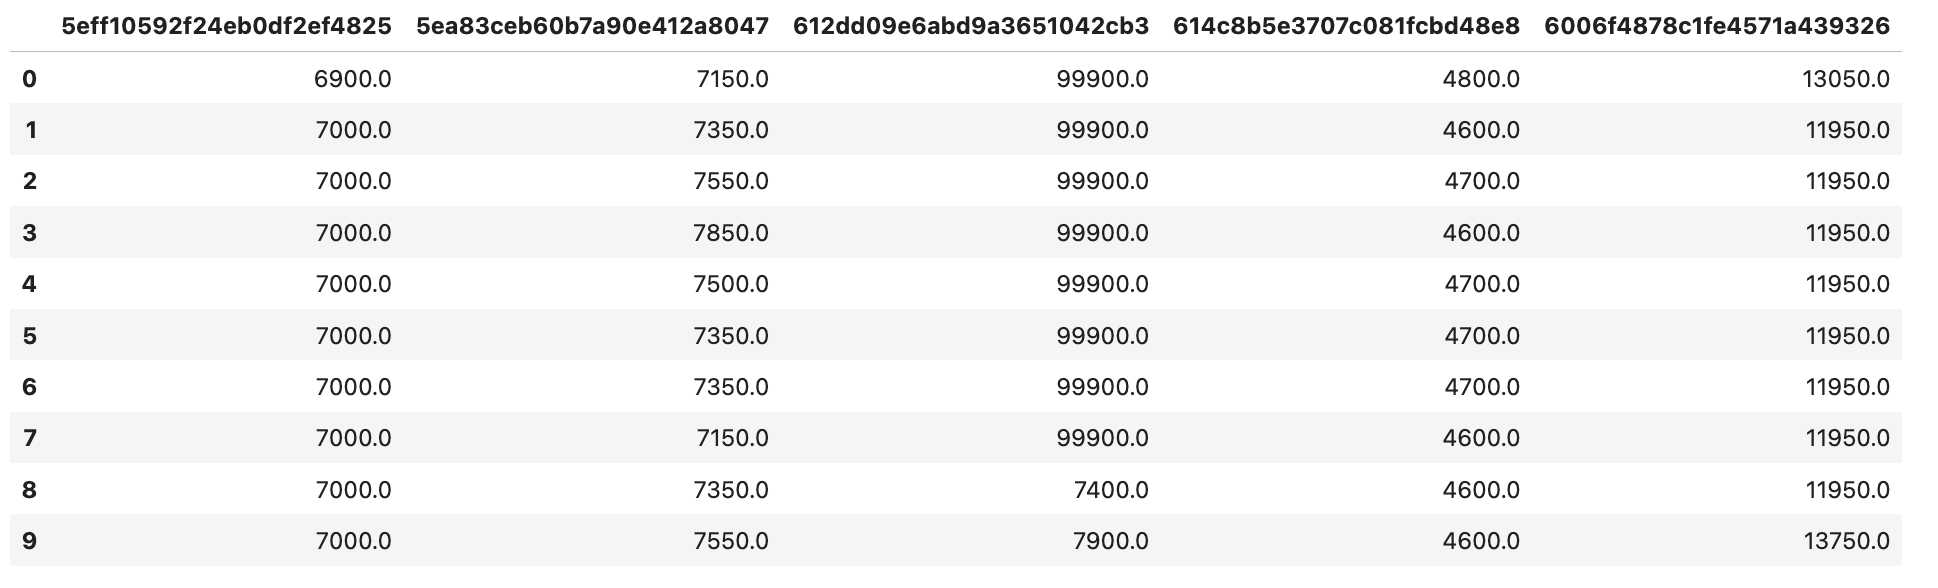
\includegraphics[width=0.9\textwidth, center]{all_prices.png}
    \caption[Preise von allen Hotels für das Jahr 2022]{Preise von allen Hotels für das Jahr 2022}
    \label{img:all_prices}
\end{figure}

Abbildung \ref{img:all_prices} zeigt einen exemplarischen Auszug aus dem DataFrame. Zudem wurde anhand diesem DataFrame noch die dazugehörige Korrelationsmatrix erstellt. Die Korrelationsmatrix ist dafür da um zusammenhänge zwischen den Vektoren zu finden. Dabei beschreibt ein Wert nahe 1 einen hohen positiven Zusammenhang der zwei Vektoren und ein Wert nahe -1 einen hohen negativen Zusammenhang der zwei Vektoren. Ein Korrelationswert gegen 0 beschreibt beschreibt keinerlei Zusammenhang der Vektoren \cite{Team.03.05.2020}. Die Vermutung ist es, dass wenn die Preise von 2 Hotels korrelieren und die Preise sich überschneiden, so werden dass ähnliche Hotels sein. 
\newline
\newline
Diese Vermutung soll dementsprechend mit einigen Hotels getestet werden:
\begin{figure}[h]
    \centering
    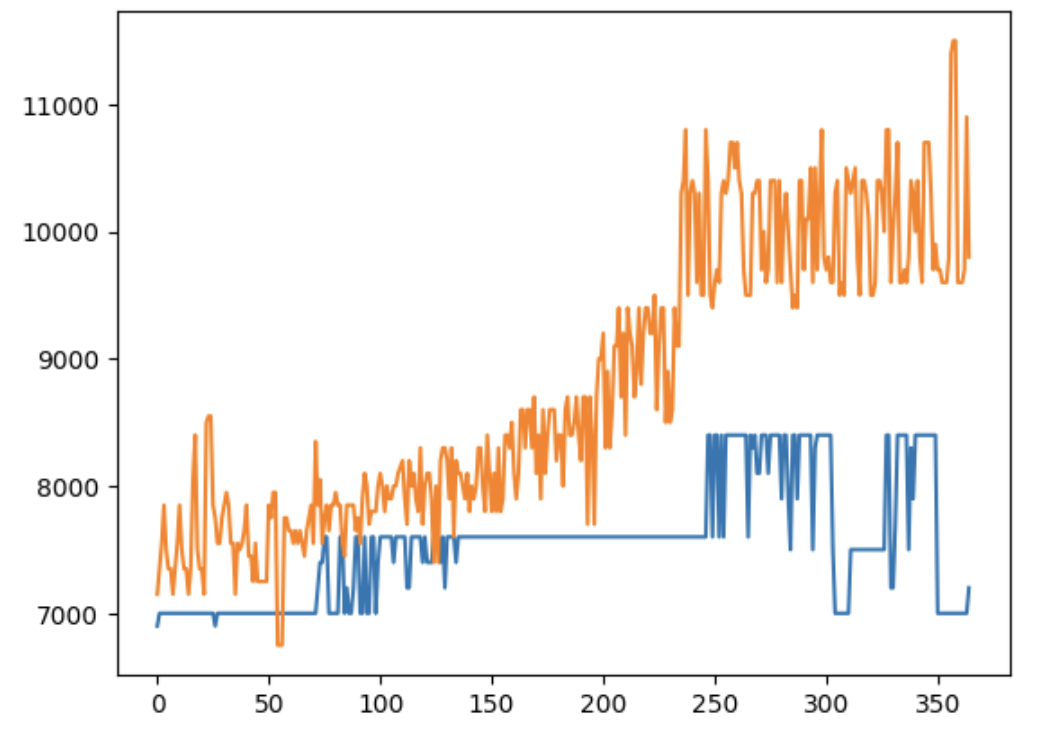
\includegraphics[width=0.9\textwidth, center]{preise_zwei_hotels.png}
    \caption[Visualisierung der Preise zweier Hotels]{Visualisierung der Preise zweier Hotels}
    \label{img:preise_zwei_hotels}
\end{figure}

\begin{figure}[h]
    \centering
    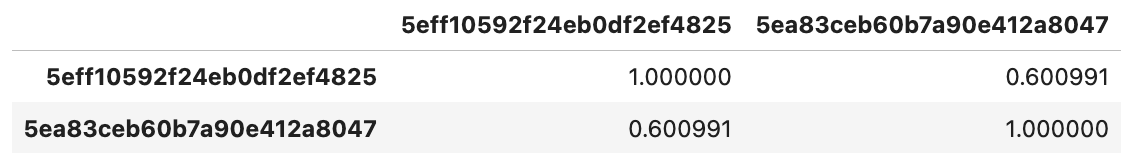
\includegraphics[width=1\textwidth, center]{corr_values_ex.png}
    \caption[Korrelationswerte der zwei Hotels]{Korrelationswerte der zwei Hotels}
    \label{img:corr_values_ex}
\end{figure}

Abbildung \ref{img:preise_zwei_hotels} illustriert den Preisverlauf von zwei Hotels im Jahr 2022, während Abbildung \ref{img:corr_values_ex} die Korrelation zwischen diesen beiden Hotels zeigt. Der festgestellte Korrelationswert von 0,6 erweist sich als bemerkenswert, insbesondere vor dem Hintergrund, dass die Preise in Abbildung \ref{img:preise_zwei_hotels} beträchtlich voneinander abweichen. Infolgedessen wurde die Überlegung angestellt, die Preise zu skalieren und daraufhin miteinander zu vergleichen. Entscheidend für ähnliche Hotels ist lediglich die Tendenz wie sich die Preise verhalten. 
\newline
\newline
Werden die Preise nun Skaliert ändert sich an der Korrelation nichts und die Skalierten Preise sehen nun wie folgt aus:

\begin{figure}[h]
    \centering
    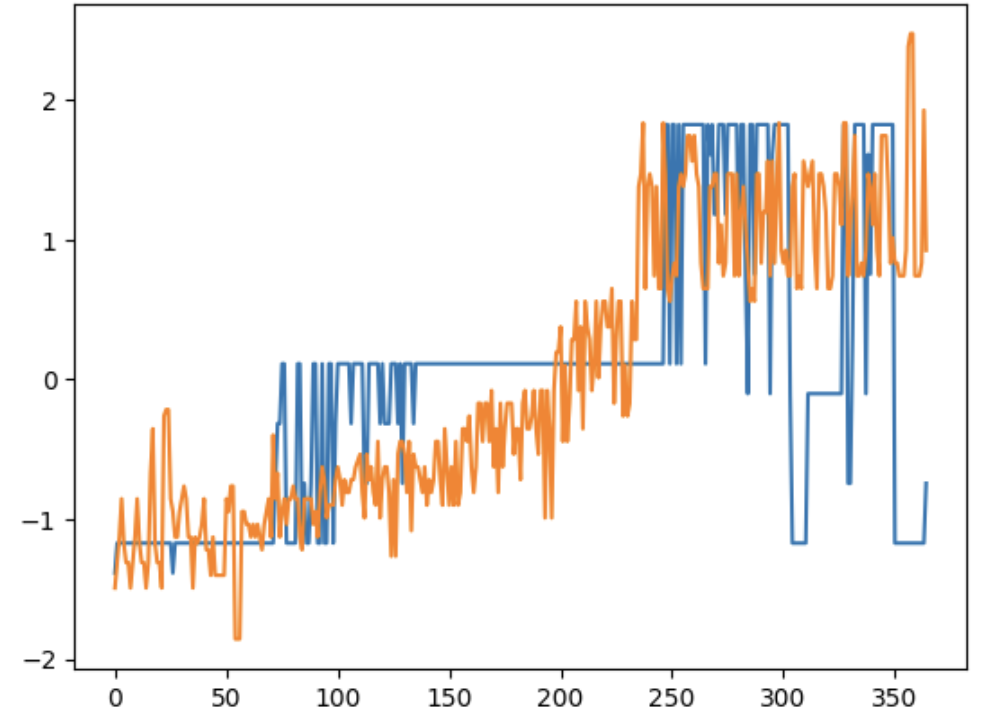
\includegraphics[width=1\textwidth, center]{scaled_preise_zwei_hotels.png}
    \caption[Visualisierung der Skalierten Preise zweier Hotels]{Visualisierung der Skalierten Preise zweier Hotels}
    \label{img:scaled_preise_zwei_hotels}
\end{figure}

Eine zusätzliche Betrachtung ergab die Frage, ob ein ähnliches Muster nicht auch durch die Verwendung des RevPAR erzielt werden könnte. Die Verwendung des RevPAR-Werts erscheint in diesem Kontext sinnvoller als die ausschließliche Berücksichtigung der Zimmerpreise, da das nachfolgende Modell letztendlich darauf abzielt, den RevPAR-Wert vorherzusagen.
\newline
\newline
Im folgenden werden die gleichen zwei Hotels mit dem RevPAR-Wert verglichen:

\begin{figure}[h]
    \centering
    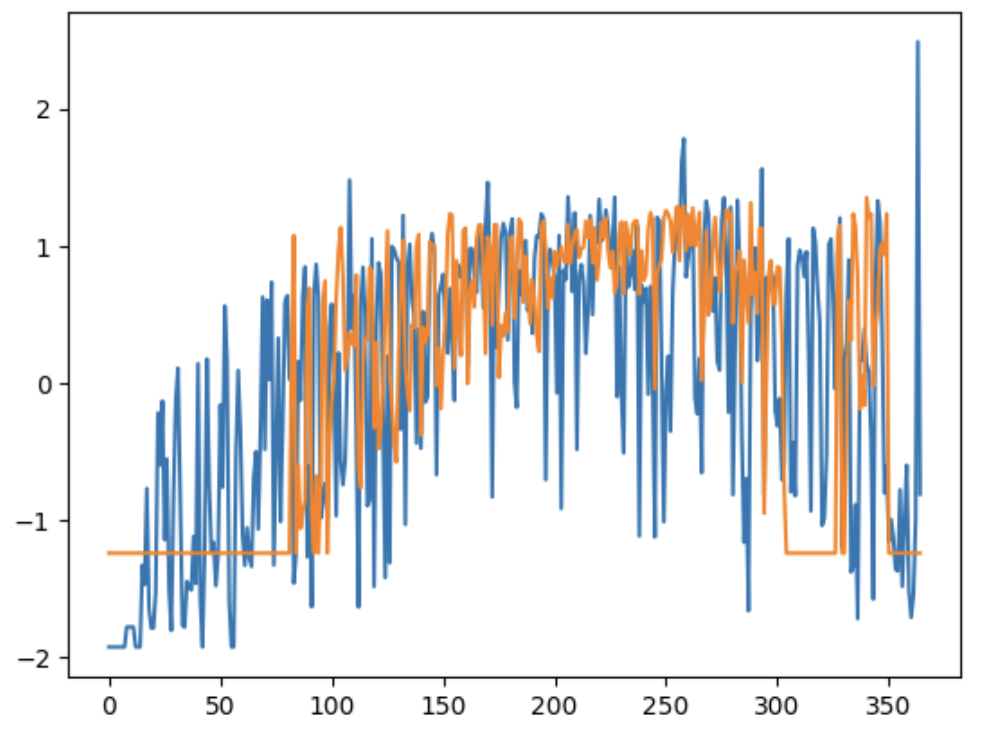
\includegraphics[width=1\textwidth, center]{scaled_revpar_zwei_hotels.png}
    \caption[Visualisierung der Skalierten RevPAR-Werte zweier Hotels]{Visualisierung der Skalierten RevPAR-Werte zweier Hotels}
    \label{img:scaled_revpar_zwei_hotels}
\end{figure}

\begin{figure}[h]
    \centering
    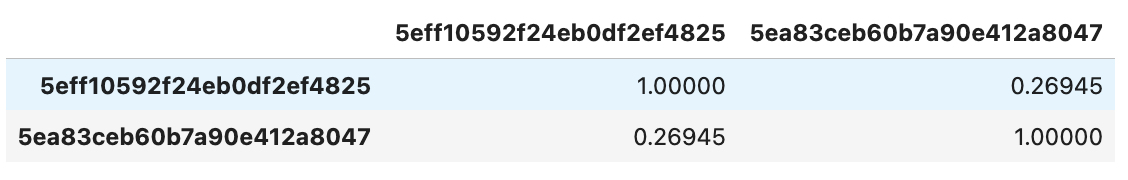
\includegraphics[width=1\textwidth, center]{corr_revpar_values_ex.png}
    \caption[Korrelationswerte der RevPAR-Werte zweier Hotels]{Korrelationswerte der RevPAR-Werte zweier Hotels}
    \label{img:corr_revpar_values_ex}
\end{figure}

Abbildung \ref{img:corr_revpar_values_ex} offenbarte einen abweichenden Korrelationswert im Vergleich zu demjenigen, der bei der Betrachtung der Preisentwicklung ermittelt wurde. Daraufhin wurde die Entscheidung getroffen, dass der Korrelationswert der RevPAR-Werte als aussagekräftiger betrachtet wird als derjenige der reinen Preisentwicklung. Infolgedessen wurde festgelegt, dass dieser Wert als Evaluation für die Ähnlichkeit zwischen den Hotels herangezogen wird.
\newline
\newline
Dieser Korrelationswert der RevPAR-Werte kann lediglich zur Evaluation der Modelle verwendet werden, da dieser Korrelationswert für ein Hotel nicht vorhanden ist. 
\chapter{Unbewachtes Lernen}
\label{subsec:un_lear}
Mit dem konstruierten Datensatz und der zusätzlichen Metrik zur Bestimmung ähnlicher Hotels erfolgt nun die Modellierung. Aufgrund der Unbekanntheit im Vorfeld, welche Hotels miteinander vergleichbar sind, wird ein Modell für unbewachtes Lernen implementiert. Unbewachtes Lernen bezeichnet eine Methode des maschinellen Lernens, bei der der Algorithmus eigenständig und ohne Überwachung Muster sowie Zusammenhänge in den Daten explorativ erkennt \cite{datasolutGmbH.05.02.2024}. Die Grundidee besteht darin, jedes Hotel in einer vergleichbaren Form dem Modell zuzuführen. Dieses Modell erkennt eigenständig Muster und Ähnlichkeiten auf Basis der gegebenen Informationen.
\newline
\newline
Die Evaluation der unterschiedlichen Ansätze und Modelle erfolgt anhand der Benchmark-Hotels, welche in der Sektion zu den Benchmark-Hotels selektiert wurden. Ein Ansatz oder Modell wird als erfolgreich betrachtet, wenn es für die Benchmark-Hotels ein oder mehrere ähnliche Hotels identifiziert, die Korrelationswert von mindestens 0,8 haben.

\subsubsection{Basismodell}
\label{subsubsec:Basismodel}
Ein Basismodell ist im Grundlegenden ein einfaches Modell, das als Referenz in einem ML-Projekt dient. Seine Hauptfunktion besteht darin, die Ergebnisse trainierter Modelle in einen Kontext zu setzen. Basismodelle sind normalerweise wenig komplex und können nur geringe Vorhersagekraft haben. Trotzdem ist ihre Einbeziehung aus verschiedenen Gründen notwendig \cite{Nair.04.04.2022}.
\newline
\newline
Einerseits dient das Basismodell dazu, einen initialen Einstieg in die Modellierung zu ermöglichen, dessen Ergebnisse anschließend mittels der zuvor ausgewählten Metrik evaluiert werden können. Hierbei wird ein vollständiger Workflow in vergleichsweise kurzer Zeit geschaffen. Andererseits fungiert das Basismodell als Referenzpunkt, welcher durch weitere Modelle übertroffen werden soll. Ein beispielhaftes Szenario für ein solches Basismodell könnte ein Empfehlungssystem für Filme sein, bei dem stets die aktuell beliebtesten Filme auf der Plattform angeboten werden.
\newline
\newline
Im vorliegenden Kontext besteht das Basismodell darin, vier zufällige Hotels aus dem Gesamtdatensatz zu extrahieren und diese als ähnlich zu betrachten. Mit dem Basismodell welches vier zufällige Hotels liefert, sieht die Evaluation wie folgt aus:

\begin{figure}[h]
    \centering
    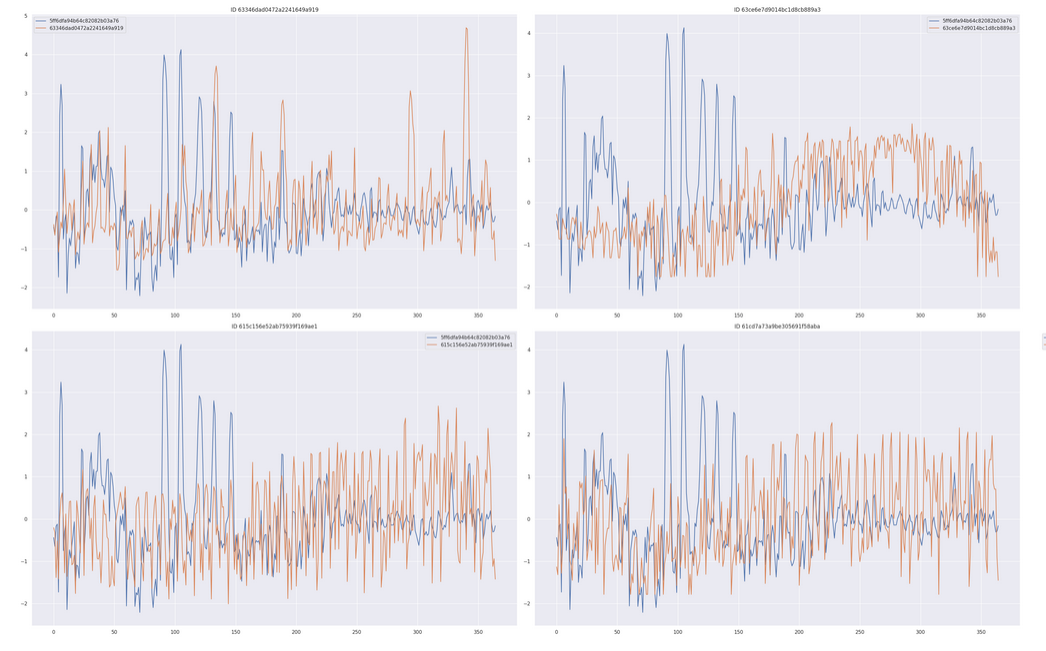
\includegraphics[width=1\textwidth, center]{basismodel_1.png}
    \caption[Basismodell Ergebnisse der RevPAR-Verläufe]{Basismodell Ergebnisse der RevPAR-Verläufe}
    \label{img:basismodell_1}
\end{figure}

\begin{figure}[h]
    \centering
    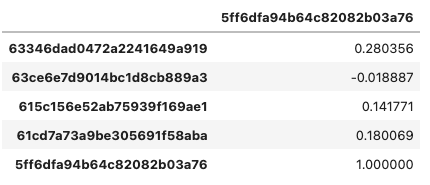
\includegraphics[width=1\textwidth, center]{basismodel_2.png}
    \caption[Basismodell Ergebnisse der RevPAR-Korrelationen]{Basismodell Ergebnisse RevPAR-Korrelationen}
    \label{img:basismodell_2}
\end{figure}

In den Abbildungen \ref{img:basismodell_1} und \ref{img:basismodell_2} sind die Ergebnisse für das Hotel mit der Identifikationsnummer \emph{5ff6dfa94b64c82082b03a76} im Zusammenhang mit dem Basismodell ersichtlich. Sowohl Abbildung \ref{img:basismodell_1} als auch Abbildung \ref{img:basismodell_2} verdeutlichen, dass die vier Hotels, welche vom Basismodell ausgewählt wurden, keine deutliche Ähnlichkeit aufweisen. Des Weiteren zeigt Abbildung \ref{img:basismodell_2} eindeutig, dass das angestrebte Ziel, ein Hotel mit einem Korrelationswert von mindestens 0,8 zu identifizieren, nicht erreicht wurde. Infolgedessen hat das Basismodell die entsprechende Anforderung nicht erfüllt.


\subsubsection{DBScan Modell}
\label{subsubsec:dbscan}
Die erste Idee nach dem Basismodell, um ähnliche Hotels zu finden, ist es den weitverbreiteten \emph{Density-Based Spatial Clustering of Applications with Noise-Algorithmus} zu nutzen. Der \emph{Density-Based Spatial Clustering of Applications with Noise-Algorithmus} kurz DBScan ist ein leistungsfähiger Ansatz zur Clusteranalyse, der darauf abzielt, Cluster in Datensätzen mit variabler Dichte zu identifizieren. Anders als klassische Clustering-Algorithmen, die auf geometrischen Formen oder Distanzmetriken basieren, nutzt DBScan die Dichte der Datenpunkte, um Cluster zu identifizieren \cite{6814687}.
\newline
\newline
Die Identifikation von Clustern innerhalb eines Datensatzes erfordert vom DBScan-Algorithmus zwei wesentliche Informationen:

\begin{itemize}
    \item Mindestanzahl an Datenpunkten für die Bildung eines Clusters.
    \item Maximale Entfernung, in der Datenpunkte voneinander liegen dürfen.
\end{itemize}

Ein Vorteil des DBScan-Algorithmus besteht darin, dass keine vorherige Festlegung darüber getroffen werden muss, wie viele Cluster am Ende resultieren sollen. Es genügt die Angabe dieser beiden genannten Informationen, um die Bildung von Clustern zu ermöglichen.
\newline
\newline
Die zugrunde liegende Hypothese dieser Methodik besagt, dass der DBScan-Algorithmus alle ähnlichen Hotels in einem Cluster zusammenführt.

\paragraph{Vorbereitung des Datensatzes} 
Der in Abbildung \ref{img:all_features_4} dargestellte Datensatz enthält sowohl numerische als auch kategoriale Daten. Da der DBScan-Algorithmus ausschließlich mit numerischen Daten arbeiten kann, ist es erforderlich, den vorhandenen Datensatz vor der Anwendung des Algorithmus zu transformieren. Zu diesem Zweck wird eine Pipeline erstellt, die auf den gesamten Datensatz angewendet wird. In einem ersten Schritt werden die kategorialen Daten mithilfe von \emph{One-Hot-Encoding} umgewandelt. Darüber hinaus erfolgt eine Skalierung der bereits vorhandenen numerischen Daten.
\newline
\newline
Die Struktur der Pipeline ist wie folgt:

\begin{lstlisting}[language=Python, label=lst:pipeline, caption=Datensatz Pipeline]
from sklearn.compose import ColumnTransformer
from sklearn.pipeline import make_pipeline
from sklearn.preprocessing import StandardScaler, OneHotEncoder

numerical_features = ['median_min', 'median_max']
categorical_features = ['art', 'region2']
    
numerical_pipeline = make_pipeline(StandardScaler())
    
categorical_pipeline = make_pipeline(OneHotEncoder())
    
preprocessor = ColumnTransformer(
    transformers=[
        ('num', numerical_pipeline, numerical_features),
        ('cat', categorical_pipeline, categorical_features)
    ])
    
    
pipeline = make_pipeline(preprocessor)
\end{lstlisting}

Die in dem Listing \ref{lst:pipeline} gezeigte Pipeline kann nun auf Datensatz angewendet werden. Dazu muss die Pipeline zunächst du den Datensatz abgestimmt werden, um dann den Datensatz zu Transformieren. Dies wird mit dem folgenden Listing veranschaulicht:

\begin{lstlisting}[language=Python, label=lst:pipeline2, caption=Ausführung der Pipeline auf dem Datensatz]
# Anpassen der Daten an die Pipeline
pipeline.fit(df)

# Transformieren der Daten
transformed_df = preprocessor.transform(df)

# Erstelle einen DataFrame aus den transformierten Daten
model_df = pd.DataFrame(transformed_df.toarray(), 
                        columns=numerical_features + 
                            list(preprocessor.named_transformers_['cat']
                                                .named_steps['onehotencoder']
                                                .get_feature_names_out(categorical_features)))
\end{lstlisting}

\paragraph{Modellbildung} 
Nach erfolgter Transformation des Datensatzes kann dieser in den DBScan-Algorithmus eingegeben werden, um die Cluster zu generieren. Als Mindestanzahl an Datenpunkten für ein Cluster wird der Wert 2 festgelegt, da stets Paare von zwei Hotels gefunden werden sollen. Das Auffinden der Cluster erfolgt daraufhin lediglich durch einen Aufruf.

\begin{lstlisting}[language=Python, label=lst:dbscan, caption=Ausführung des DBScan-Algorithmus]
from sklearn.cluster import DBSCAN

# Define variables
eps = 0.8
min_samples = 2 

# Create the DBScan algorithm
dbscan = DBSCAN(eps=eps, min_samples=min_samples)

# Add Cluster to df
model_df['Cluster'] = dbscan.fit_predict(model_df)
\end{lstlisting}

Das Listing \ref{lst:dbscan} veranschaulicht die Initialisierung des DBScan-Algorithmus sowie die Erzeugung der individuellen Cluster. Diese Cluster werden anschließend der Datenreihe in der Spalte \emph{Cluster} zugeordnet.
\newline
\newline
In einem nachfolgenden Schritt können die erstellten Cluster wie folgt visualisiert werden:

\begin{figure}[h]
    \centering
    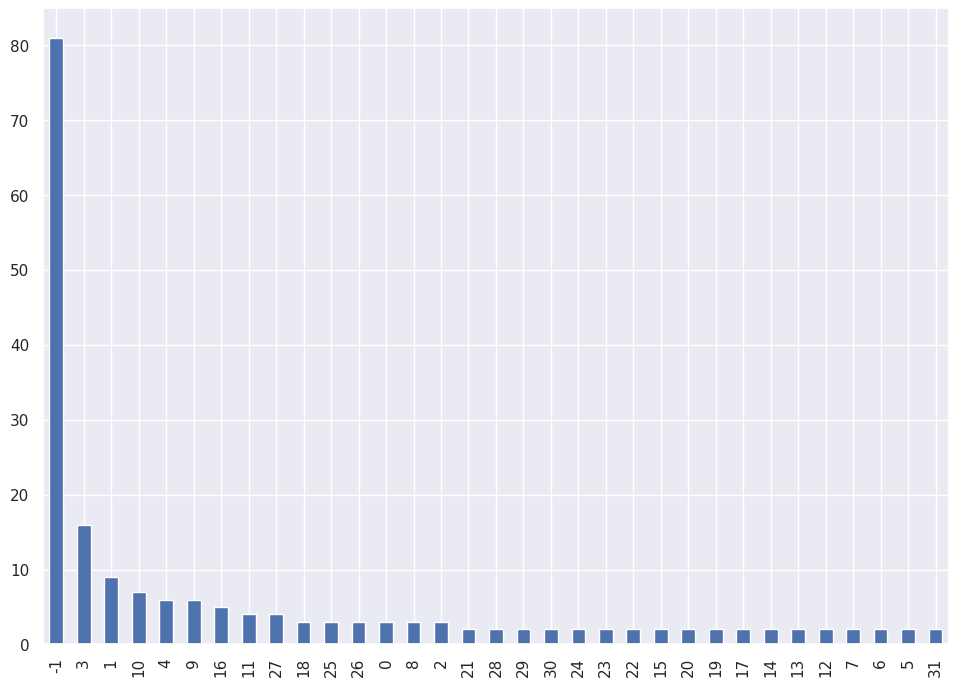
\includegraphics[width=0.85\textwidth, center]{cluster.png}
    \caption[DBScan Clusters]{DBScan Clusters}
    \label{img:cluster}
\end{figure}

Abbildung \ref{img:cluster} zeigt die verschiedenen Cluster, die durch den DBScan-Algorithmus erstellt wurden. Es sind insgesamt 32 Cluster zu erkennen, beginnend mit Cluster 0, sowie eine weitere Kategorie \emph{-1}, die anzeigt, dass für diese Hotels kein Cluster gefunden wurde. Bemerkenswert ist dabei, dass die Mehrheit dieser Hotels keinem Cluster zugeordnet wurde.
\newline
\newline
Ungeachtet dieser Beobachtung soll im nächsten Schritt überprüft werden, welche Hotels mit dem Benchmark-Hotel in einem Cluster vorhanden sind. Hierfür müssen die Hotel-IDs in einer zusätzlichen Spalte dem Dataframe hinzugefügt werden. Die nachfolgende Code-Sequenz im angegebenen Listing ermöglicht die Identifikation der Hotels, die mit dem Benchmark-Hotel in einem Cluster sind.

\begin{lstlisting}[language=Python, label=lst:dbscan_values, caption=Finden alle Hotel ID´s innerhalb des gleichen Clusters]
# Add hotel ids to the dataset with the clusters
model_df['hotel_id'] = df.index

# Get the row for the benchmark hotel
benchmark_row = model_df[model_df["hotel_id"] == str(benchmark_hotel_id)]

# Get the Cluster value of the benchmark hotel
benchmark_cluster = list(benchmark_row["Cluster"].values)[0]

# Get the rows with the same cluster as the benchmark hotel
benchmark_cluster_df = model_df[model_df["Cluster"] == benchmark_cluster]

# Get the hotel ids 
hotel_ids = list(benchmark_cluster_df["hotel_id"].values)
\end{lstlisting}

Die Variable \emph{hotel\_ids} enthält nun sämtliche Hotel-IDs, die zusammen mit dem Benchmark-Hotel in einem Cluster verortet sind. Initial besteht das Interesse darin, die identifizierten Hotels zu visualisieren. Daher soll im Anschluss angezeigt werden, welche Merkmale die identifizierten Hotels aufweisen.

\begin{figure}[h]
    \centering
    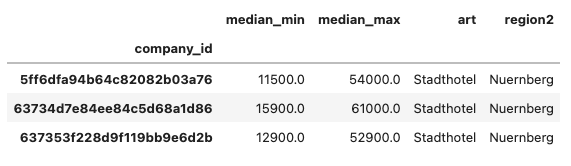
\includegraphics[width=1\textwidth, center]{dbscan_hotels_1.png}
    \caption[Gefundene Hotels für das erste Benchmark-Hotel mit dem DBScan-Algorithmus]{Gefundene Hotels für das erste Benchmark-Hotel mit dem DBScan-Algorithmus}
    \label{img:dbscan_hotels_1}
\end{figure}

Die Hotels, die im identifizierten Cluster zu finden sind, weisen tatsächlich Ähnlichkeiten zu den Merkmalen auf, die das Benchmark-Hotel mit der ID \emph{5ff6dfa94b64c82082b03a76} charakterisieren. Da die Aussagekraft eines einzelnen Hotels begrenzt ist, soll das zweite Benchmark-Hotel ebenfalls mit einbezogen werden. Hierbei sollen auch für dieses Hotel zunächst die identifizierten Hotels anhand ihrer Merkmale bewertet werden.

\begin{figure}[h]
    \centering
    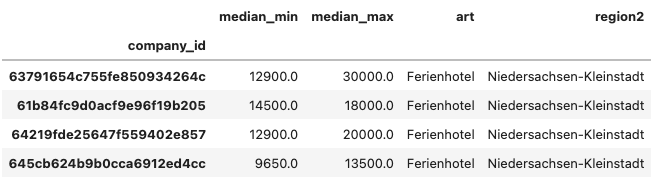
\includegraphics[width=1\textwidth, center]{dbscan_hotels_2.png}
    \caption[Gefundene Hotels für das zweite Benchmark-Hotel mit dem DBScan-Algorithmus]{Gefundene Hotels für das zweite Benchmark-Hotel mit dem DBScan-Algorithmus}
    \label{img:dbscan_hotels_2}
\end{figure}

Unter Berücksichtigung des zweiten Hotels wird ersichtlich, dass der DBScan Hotels mit ähnlichen Merkmalen identifiziert. Dennoch lässt sich anhand der vorliegenden Merkmale nicht eindeutig feststellen, ob diese Hotels tatsächlich ähnliche Verläufe in Bezug auf den RevPAR aufweisen.

\paragraph{Evaluation}
Angesichts der Tatsache, dass allein anhand der Merkmale keine klare Aussage über die tatsächliche Ähnlichkeit der Hotels getroffen werden kann, erfolgt in der nachfolgenden Sektion eine Evaluierung der beiden Benchmark-Hotels. 
\newline
\newline
Der Beginn dieser Evaluierung erfolgt mit dem Hotel, das die ID \emph{5ff6dfa94b64c82082b03a76} trägt. Die Ergebnisse dieser Evaluation werden im Folgenden dargestellt:

\begin{figure}[h]
    \centering
    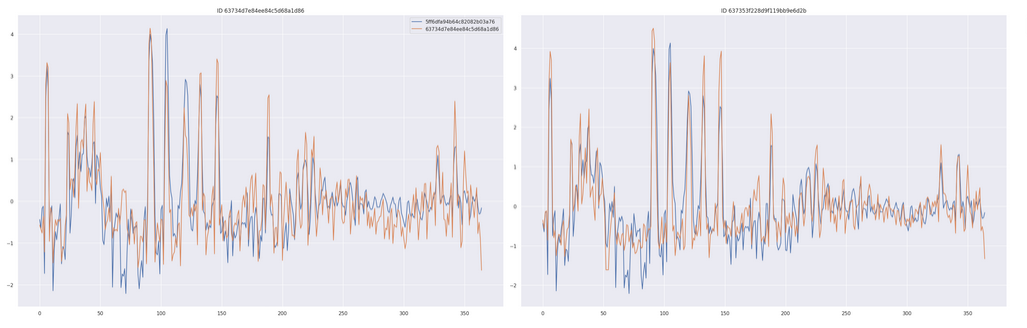
\includegraphics[width=1\textwidth, center]{dbscan_results_1.png}
    \caption[DBScan Ergebnisse der RevPAR-Verläufe für das erste Benchmark-Hotel]{DBScan Ergebnisse der RevPAR-Verläufe für das erste Benchmark-Hotel}
    \label{img:dbscan_results_1}
\end{figure}

\begin{figure}[h]
    \centering
    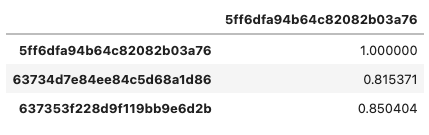
\includegraphics[width=1\textwidth, center]{dbscan_results_1_1.png}
    \caption[DBScan Ergebnisse der RevPAR-Korrelationen für das erste Benchmark-Hotel]{DBScan Ergebnisse der RevPAR-Korrelationen für das erste Benchmark-Hotel}
    \label{img:dbscan_results_1_1}
\end{figure}

Die Abbildungen \ref{img:dbscan_results_1} und \ref{img:dbscan_results_1} verdeutlichen, dass die identifizierten Hotels die Voraussetzungen für einen Korrelationswert von mindestens 0,8 erfüllen. Die Ergebnisse für das Hotel mit der ID \emph{5ff6dfa94b64c82082b03a76} erweisen sich demnach als zufriedenstellend. Allerdings ist eine gewisse Skepsis angebracht, da es auch rein zufällig sein könnte, dass diese Hotels Ähnlichkeiten in Bezug auf den RevPAR Verlauf aufweisen. Aus diesem Grund soll die gleiche Evaluation auch mit dem zweiten Hotel, welches die ID \emph{645cb624b9b0cca6912ed4cc} trägt, durchgeführt werden.

\begin{figure}[h]
    \centering
    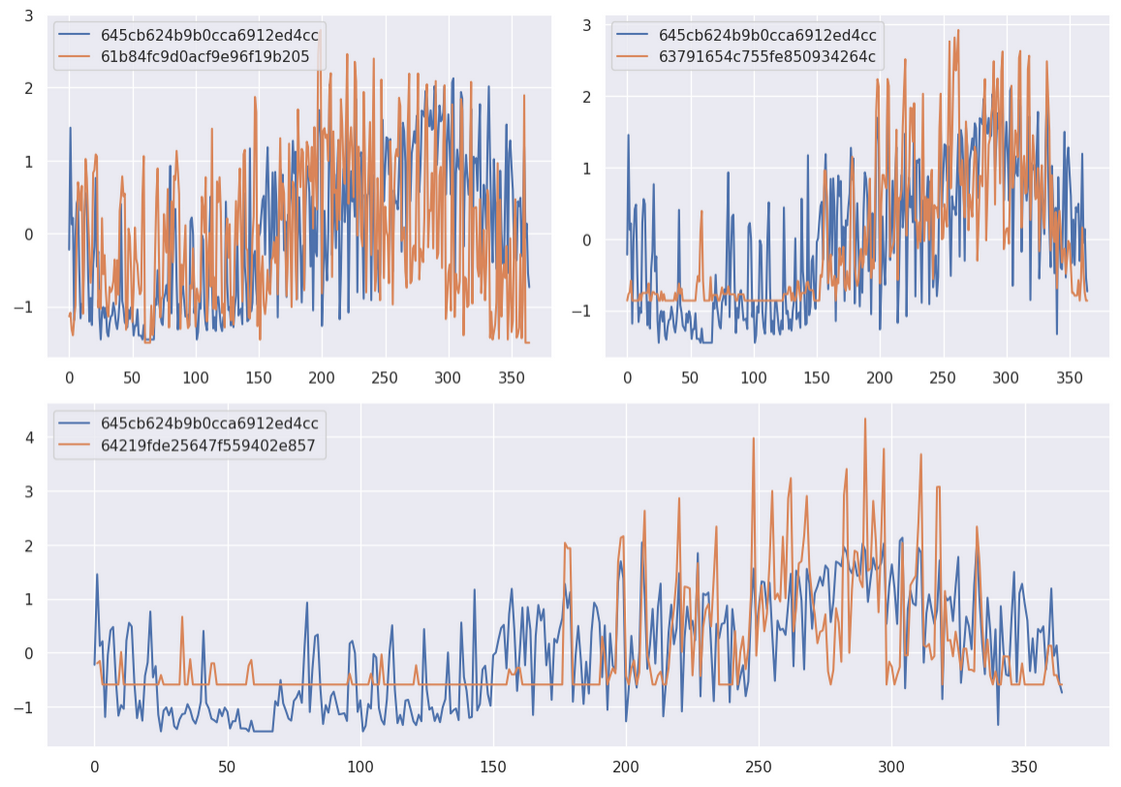
\includegraphics[width=1\textwidth, center]{dbscan_results_2.png}
    \caption[DBScan Ergebnisse der RevPAR-Verläufe für das zweite Benchmark-Hotel]{DBScan Ergebnisse der RevPAR-Verläufe für das zweite Benchmark-Hotel}
    \label{img:dbscan_results_2}
\end{figure}

\begin{figure}[h]
    \centering
    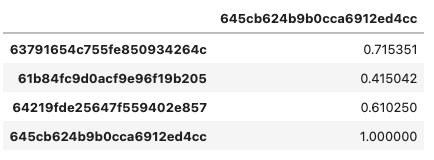
\includegraphics[width=1\textwidth, center]{dbscan_results_2_1.png}
    \caption[DBScan Ergebnisse der RevPAR-Korrelationen für das zweiten Benchmark-Hotel]{DBScan Ergebnisse der RevPAR-Korrelationen für das zweite Benchmark-Hotel}
    \label{img:dbscan_results_2_1}
\end{figure}

Die Evaluation des Hotels mit der ID \emph{645cb624b9b0cca6912ed4cc} ergab, dass die Anforderungen an einen Korrelationswert von mindestens 0,8 nicht erfüllt wurden. Somit lässt sich ableiten, dass die Ähnlichkeit der Merkmale zwischen den einzelnen Hotels nicht zwangsläufig mit der Ähnlichkeit in Bezug auf die RevPAR-Werte in Verbindung steht. 
\newline
\newline
Obwohl der DBScan-Algorithmus im Vergleich zum Basismodell verbesserte Ergebnisse lieferte, bleibt das Gesamtergebnis dennoch unbefriedigend. Besonders bedenklich ist dabei, dass die überwiegende Mehrheit der Hotels keinem Cluster zugeordnet werden konnten.


\section{Doc2Vec Modell}
\label{subsubsec:doc2vec}
In Anbetracht des unbefriedigenden Ergebnisses des DBScan-Algorithmus wird nun die Erprobung eines weiteren Modells in Betracht gezogen, um ähnliche Hotels zu identifizieren. Die nächste Alternative besteht in der Anwendung des Doc2Vec-Modells.
\newline
\newline
Doc2Vec ist ein maschinelles Lernverfahren, das dazu dient, Dokumente in einem kontinuierlichen Vektorraum abzubilden. Es wurde als Weiterentwicklung von Word2Vec konzipiert, einem etablierten Ansatz zur Repräsentation von Wörtern in einem semantischen Vektorraum. Das Hauptziel von Doc2Vec besteht darin, eine kontinuierliche Darstellung von Dokumenten zu generieren, um semantische Ähnlichkeiten zwischen diesen Dokumenten zu erfassen \cite{LeV.16.05.2014}.
\newline
\newline
Die grundlegende Idee besteht darin, jedes Hotel in einem textbasierten Dokument zu repräsentieren und dem Doc2Vec-Modell die Aufgabe zu übertragen, ähnliche Dokumente zu identifizieren. Dieser Ansatz zielt darauf ab, zu verhindern, dass Hotels ohne jegliche Zuordnung zu anderen Hotels vorliegen.
\newline
\newline
Ähnlich wie beim DBScan, wo der Vorteil darin bestand, keine Cluster angeben zu müssen, weist auch das Doc2Vec-Modell den Vorteil auf, dass keinerlei Cluster explizit angegeben werden müssen. Zudem eröffnet sich hier ein weiterer Vorteil, der beim DBScan-Algorithmus nicht gegeben war. Die beiden Informationen \emph{Art} und \emph{Region} sind beide durch Strings repräsentiert. Da Doc2Vec mit einer textbasierten Repräsentation arbeitet, bedarf es keiner Umwandlung dieser beiden Merkmale mittels \emph{One-Hot-Encoding}.

\subsection{Vorbereitung des Datensatzes} 
Auch in diesem Kontext erfordert der in Abbildung \ref{img:all_features_4} dargestellte Datensatz eine vorherige Verarbeitung, um mit dem Doc2Vec-Modell kompatibel zu sein. Die Vorbereitung besteht darin, dem Datensatz eine zusätzliche Spalte hinzuzufügen, die sämtliche Informationen des Hotels als textbasiertes Dokument repräsentiert. 
\newline
\newline
Im Folgenden wird eine Hilfsfunktion präsentiert, die dazu dient, die textbasierten Dokumente anhand der einzelnen Informationen zu erstellen.

\begin{lstlisting}[language=Python, label=lst:doc2vec_hilfs_func, caption=Hilfsfunktion zur Erzeugung von textbasierten Dokumenten]
# Copy the dataset to keep the original clean
doc2vec_df = df.copy()
    
# Get the columns of the dataset dynamic
column_names = doc2vec_df.columns
    
# Function to generate the document out of each columns
def concatenate_columns(row):
    result = "Hoteleigenschaften: "
    for column in column_names:
        result += column + "=" + str(row[column]) + " "
    return result
    
# Add the document in a new column "doc"
doc2vec_df['doc'] = doc2vec_df.apply(concatenate_columns, axis=1)
\end{lstlisting}

Durch die im Listing \ref{lst:doc2vec_hilfs_func} präsentierten Codezeilen, wurde dem Datensatz eine neue Spalte namens \emph{doc} hinzugefügt, die später als Eingabe für das Modell dienen soll. Zur Veranschaulichung dieser neu erstellten \emph{doc}-Spalte soll das erste Dokument als Beispiel dienen:

\begin{figure}[h]
    \centering
    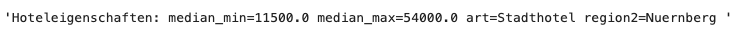
\includegraphics[width=1\textwidth, center]{ex_doc.png}
    \caption[Exemplarisches Dokument innerhalb des Datensatzes]{Exemplarisches Dokument innerhalb des Datensatzes}
    \label{img:ex_doc}
\end{figure}

Mithilfe dieser neuen Repräsentation kann nun im nächsten Schritt das Modell trainiert werden.

\subsection{Modellbildung}

Nach der erfolgten Datenvorbereitung und der Erstellung der textbasierten Dokumente für jedes Hotel kann das Modell nun trainiert werden. Hierzu werden die Hotel-IDs zunächst als Index festgelegt. Anschließend wird der Datensatz in sogenannte \emph{TaggedDocument} Objekte umgewandelt. Diese \emph{TaggedDocument} Objekte erfassen die einzelnen Wörter innerhalb eines Dokuments sowie ein sogenanntes \emph{Tag}, welches zur Identifikation des jeweiligen Dokuments dient. In diesem Kontext repräsentiert das \emph{Tag} die Hotel-ID. Der letzte Schritt besteht darin, die \emph{TaggedDocument} Objekte unter Verwendung einiger Hyperparameter dem Modell zuzuführen und das Training zu starten. Sobald das Modell trainiert ist, können ähnliche Dokumente zu einem ausgewählten Dokument, das durch die Hotel-ID identifiziert wird, gefunden werden.
\newline
\newline
Dieses Verhalten wird im nachfolgenden Listing dargestellt:
\begin{lstlisting}[language=Python, label=lst:doc2vec_exe, caption=Ausführung des Doc2Vec Modell]
# Generate the TaggetDocuments with Hotel-ID as Tag
documents = [TaggedDocument(words=doc.split(), tags=[str(i)]) for i, doc in doc2vec_df["doc"].iteritems()]
    
# Train the Model
model = Doc2Vec(documents, vector_size=10, window=3, min_count=1, workers=4, epochs=1000, alpha=0.01)
    
# Get similar documents als tupel (ID, Doc)
similar_documents = model.dv.most_similar(str(benchmark_hotel_id), topn=4)
    
pred_hotel_ids = [tupel[0] for tupel in similar_documents]
\end{lstlisting}

Nun stehen in der Variable \emph{pred\_hotel\_ids} die Hotel-IDs, die anhand von dem Doc2Vec Modell als am ähnlichsten empfunden wurden. Diese können wie auch schon beim DBScan Algorithmus anhand ihrer Merkmale betrachtet werden.

\begin{figure}[h]
    \centering
    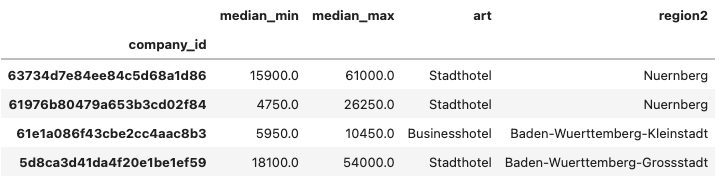
\includegraphics[width=1\textwidth, center]{doc2vec_hotels_1.png}
    \caption[Gefundene Hotels für das erste Benchmark-Hotel mit dem Doc2Vec Modell]{Gefundene Hotels für das erste Benchmark-Hotel mit dem Doc2Vec Modell}
    \label{img:doc2vec_hotels_1}
\end{figure}

Es zeigt sich, dass das Doc2Vec Modell ganz andere Hotels als ähnlich identifiziert hat. Im Gegensatz zum DBScan-Algorithmus scheinen die Merkmale der gefundenen Hotels lediglich Überlappungen aufzuweisen, anstatt sich zu teilen. Wie bereits in den vorhergehenden Abschnitten ersichtlich wurde, müssen sich die Merkmale nicht zwangsläufig überschneiden.

\subsection{Evaluation}
Ungeachtet der jeweiligen Merkmale der einzelnen Hotels besteht die Möglichkeit, dass diese dennoch Ähnlichkeiten in dem RevPAR-Verlauf aufweisen. Diese Annahme soll im Folgenden überprüft werden.

\begin{figure}[h]
    \centering
    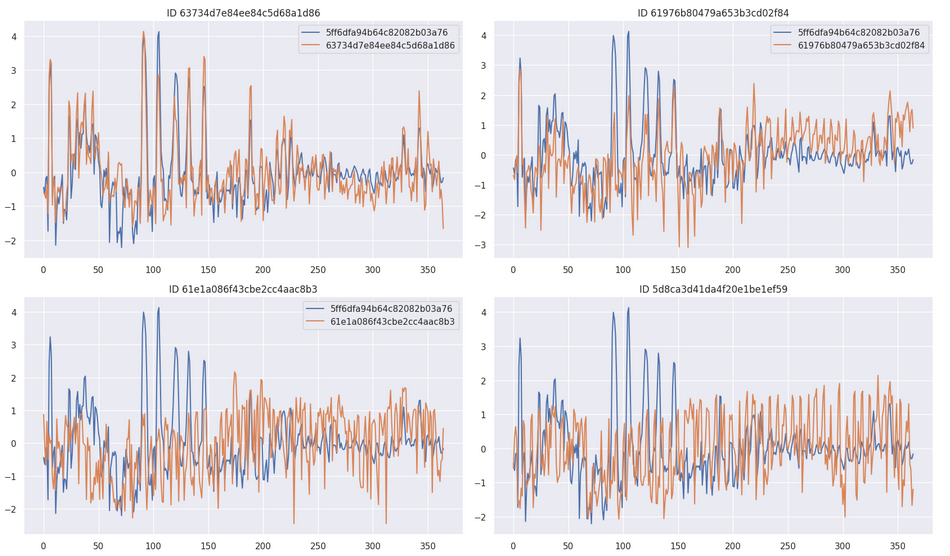
\includegraphics[width=1\textwidth, center]{doc2vec_results_1.png}
    \caption[Doc2Vec Ergebnisse der RevPAR-Verläufe für das erste Benchmark-Hotel]{Doc2Vec Ergebnisse der RevPAR-Verläufe für das erste Benchmark-Hotel}
    \label{img:doc2vec_results_1}
\end{figure}

\begin{figure}[h]
    \centering
    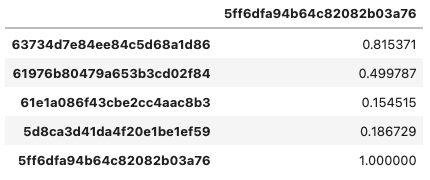
\includegraphics[width=0.5\textwidth, center]{doc2vec_results_1_1.png}
    \caption[Doc2Vec Ergebnisse der RevPAR-Korrelationen für das erste Benchmark-Hotel]{Doc2Vec Ergebnisse der RevPAR-Korrelationen für das erste Benchmark-Hotel}
    \label{img:doc2vec_results_1_1}
\end{figure}

Es offenbart sich, dass das Doc2Vec-Modell erheblich schlechter abschneidet als der DBScan-Algorithmus. Diese Feststellung wird bereits anhand des ersten Benchmark-Hotels ersichtlich, und es wird daher auf die detaillierte Evaluation dieses Benchmark-Hotels verzichtet.
\subsubsection{Unbewachtes Lernen Fazit}
\label{subsubsec:un_fazit}
Sowohl der Einsatz des DBScan-Algorithmus als auch der Ansatz des Doc2Vec-Modells haben sich als unzureichend erwiesen. Trotz der Identifikation von Hotels in beiden Ansätzen lässt sich im Vorfeld nicht sicherstellen, ob diese tatsächlich als ähnlich zueinander betrachtet werden können. Aufgrund dieser Erkenntnisse wurde die Entscheidung getroffen, beide Ansätze zu verwerfen und eine neue Methodik zur Identifizierung ähnlicher Hotels zu entwickeln.
\subsection{Überwachtes Lernen}
\label{subsec:lean}
Beide unbewachte Ansätze erwiesen sich als nicht zufriedenstellend, dennoch haben sie wertvolle Erkenntnisse geliefert. Es wurde festgestellt, dass die erforderlichen Korrelationswerte für eine Evaluierung vorhanden sind, mit Ausnahme von neuen Hotels ohne entsprechende Daten. Nichtsdestotrotz könnten die bestehenden Korrelationswerte trotzdem genutzt werden, um ein Modell zu trainieren. Die Idee besteht darin, die beschreibenden Merkmale eines Hotels in ein trainiertes Modell einzuspeisen, um die Korrelationswerte vorherzusagen, anstatt direkt ähnliche Hotels zu prognostizieren.
\newline
\newline
Konkret sieht der Ansatz wie folgt aus: Jedes Hotel im Datensatz wird mit jedem anderen Hotel kombiniert, wodurch ein Datensatz der Größe \emph{Anzahl der Hotels x Anzahl der Hotels} entsteht. Zu jeder Kombination wird der Korrelationswert in einer separaten Spalte hinzugefügt, die als Zielvariable für die Vorhersage dient. Ein Modell wird mithilfe dieser Daten und der jeweiligen Zielvariable trainiert. Bei der Vorhersage der Korrelationswerte für ein neues Hotel wird dieses mit jedem anderen Hotel kombiniert und in das Modell eingebracht. Das Modell gibt schließlich die vorhergesagten Korrelationswerte aus.
\newline
\newline
Um diese theoretische Idee zu konkretisieren, werden im folgenden Abschnitt die einzelnen Schritte veranschaulicht.

\subsubsection{Vorbereitung des Datensatzes}
\label{subsubsec:learn_prepare}
Um die beschriebene Idee in die Tat umzusetzen, bedarf es zunächst einer Modifikation des Datensatzes, welcher in Abbildung \ref{img:all_features_4} dargestellt ist. Jede Zeile soll mit jeder anderen Zeile kombiniert werden. Dies wird durch die nachfolgenden Codezeilen realisiert:

\begin{lstlisting}[language=Python, label=lst:learn_prepare, caption=Erstellen des kombinierten Datensatzes]
# Get Hotel ID as seperate column
model_df = model_df.reset_index()
    
# Repeat the rows 2 times
repeat = 2
    
# Get all row combinations 
combinations = list(product(model_df.index, repeat=repeat))
    
# Create the empty result dataframe
combined_df = pd.DataFrame(columns=[f"{column}_{i+1}" for i in range(repeat) for column in model_df.columns])
    
# Combine all combinations in the result dataframe
for combination in combinations:
    row1 = model_df.iloc[combination[0]].values
    row2 = model_df.iloc[combination[1]].values
    new_row = pd.Series(list(row1) + list(row2), index=combined_df.columns)
    combined_df = combined_df.append(new_row, ignore_index=True)
\end{lstlisting}

Mithilfe der im Listing \ref{lst:learn_prepare} präsentierten Codezeilen wurden sämtliche Zeilen erfolgreich miteinander kombiniert. Anschließend kann der Korrelationswert jeder Kombination als neue Spalte \emph{target} hinzugefügt werden.
\newline
\newline
Der resultierende Datensatz, welcher für das Modell verwendet werden soll, sieht wie folgt aus\footnote{Die Hotel-IDs wurden zur besseren Veranschaulichung entfernt}:

\begin{figure}[h]
    \centering
    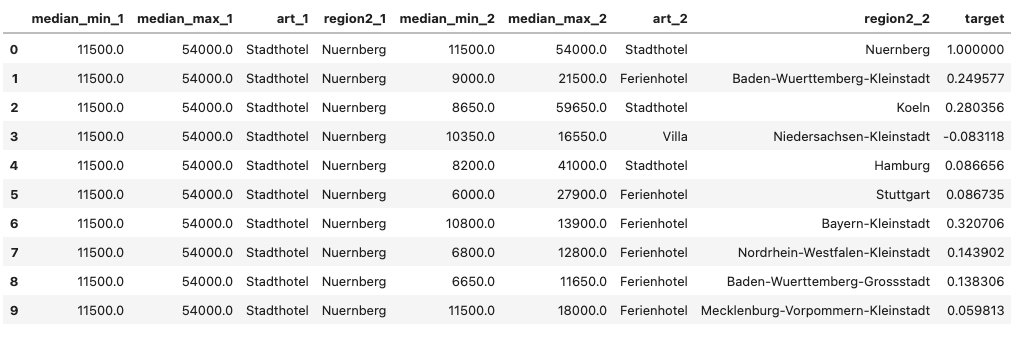
\includegraphics[width=1\textwidth, center]{learn_df1.png}
    \caption[Datensatz bestehend aus den einzelnen Kombinationen]{Datensatz bestehend aus den einzelnen Kombinationen}
    \label{img:learn_df1}
\end{figure}

\subsubsection{Modellbildung}
\label{subsubsec:learn_model}
Für das überwachte Lernen wird CatBoost verwendet, ein hochentwickelter Machine-Learning-Algorithmus, der gezielt auf die Vorhersage von kategorialen Variablen in Datensätzen abzielt und auf dem Gradient Boosting Framework basiert. Eine signifikante Eigenschaft von CatBoost ist seine einzigartige Methode zur Behandlung von kategorialen Merkmalen, bekannt als \emph{Kategorie-Binning}. Diese Methode befähigt den Algorithmus dazu, die internen Strukturen kategorialer Variablen besser zu erfassen und sie effektiv in den Trainingsprozess einzubeziehen, was zu präziseren Vorhersagen führt \cite{Hancock.2020}.
\newline
\newline
Angesichts der Fülle an kategorialen Variablen im vorliegenden Datensatz erweist sich der CatBoost-Algorithmus als besonders geeignet für diese spezifische Aufgabe. Demzufolge kann der Datensatz in seiner aktuellen Form verwendet werden, ohne dass eine umfangreiche Vorverarbeitung erforderlich ist.
\newline
\newline
Im folgenden Abschnitt werden die erforderlichen Codezeilen präsentiert, um das Modell zu trainieren und Vorhersagen für das Benchmark-Hotel zu generieren:

\begin{lstlisting}[language=Python, label=lst:learn_model_train, caption=Erzeugung der Vorhersagen von ähnlichen Hotels mittels CatBoost]
# Get test data
test = combined_df[combined_df["company_id_1"] == str(benchmark_hotel_id)]
# Get train data
train = combined_df.drop(combined_df[(combined_df["company_id_1"] == str(benchmark_hotel_id)) | (combined_df["company_id_2"] == str(benchmark_hotel_id))].index)
# Get X and y from test and train
y_train = train["target"]
X_train = train.drop("target", axis=1)
y_test = test["target"]
X_test = test.drop("target", axis=1)
# Save important informations
hotel_test_df = X_test[["company_id_1", "company_id_2"]]
hotel_test_df["target"] = list(y_test)
# Drop Company ID
X_train = X_train.drop(['company_id_1', "company_id_2"], axis=1)
X_test = X_test.drop(['company_id_1', "company_id_2"], axis=1)
# Define cat features 
cat_features = ["art_1", "region2_1", "art_2","region2_2"]
# Define and train model 
model = cb.CatBoostRegressor()
model.fit(X_train, y_train, cat_features=cat_features)
# Get predictions 
y_pred = model.predict(X_test)
# Add predictions to the information df
hotel_test_df["predictions"] = list(y_pred)
\end{lstlisting}

Mithilfe der Codezeilen im Listing \ref{lst:learn_model_train} wurde ein zusätzliches DataFrame erstellt, das die Hotel-IDs sowie deren Vorhersagen enthält. Dieses DataFrame wird im Folgenden präsentiert:

\begin{figure}[h]
    \centering
    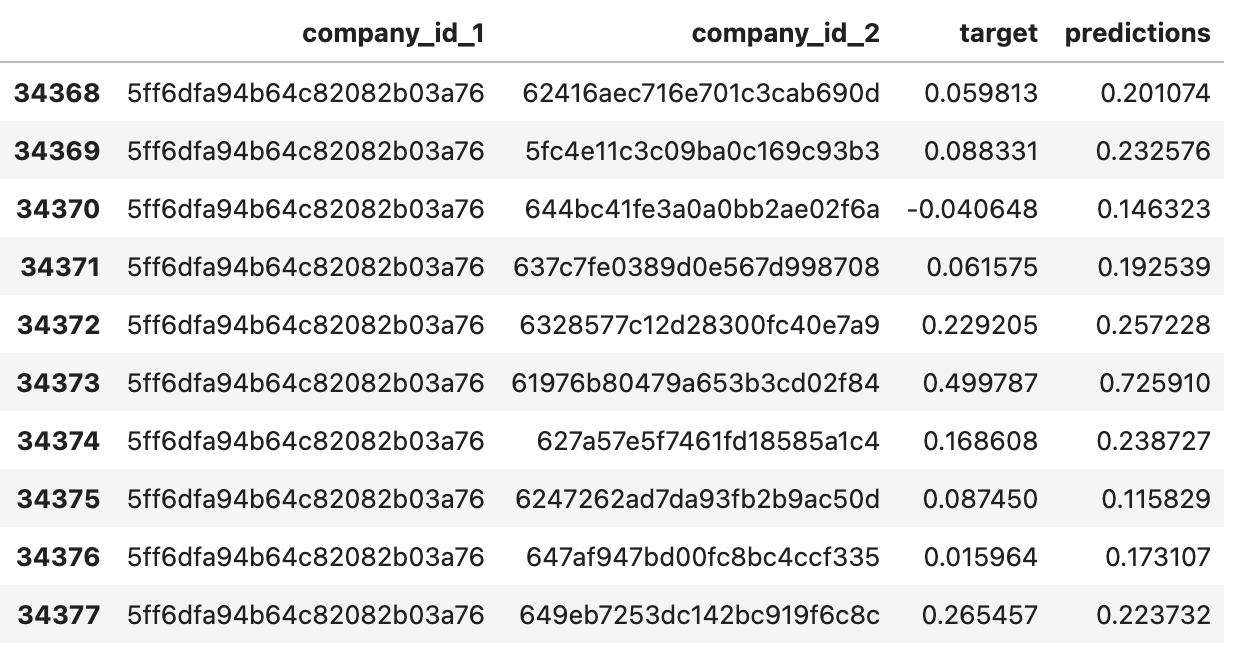
\includegraphics[width=1\textwidth, center]{catboost_similar_results.png}
    \caption[Datensatz der Hotel-IDs und deren Korrelationswert]{Datensatz der Hotel-IDs und deren Korrelationswert}
    \label{img:catboost_similar_results}
\end{figure}

Es besteht nun die Möglichkeit, verschiedene Operationen auf dem DataFrame auszuführen. Zum Beispiel kann auf dem DataFrame gemäß der Bedingung in Abschnitt \emph{\nameref{subsec:un_lear}} gefiltert werden, die besagt, dass Hotelkorrelationen mit mindestens einem Korrelationswert von 0,8 gefunden werden sollen.

\subsubsection{Evaluation}
\label{subsubsec:learn_eval}
Im Gegensatz zu früheren Modellen wurde bei diesem Modell auf eine umfassende Evaluation verzichtet, da der prognostizierte Korrelationswert ausreichend ist, um ähnliche Hotels zu identifizieren. Es wurde lediglich versucht, den R2-Score mithilfe von Hyperparameteranalysen mittels Random Search 
\cite{AdapRandomSearch4.05.2009} und Grid Search \cite{Liashchynskyi.12.12.2019} zu verbessern.



\section{Finden von ähnlichen Hotels Fazit}
\label{subsec:similar_fazit}
In dieser Sektion wurden verschiedene Ansätze zum Finden von ähnlichen Hotels erforscht, beginnend mit dem Einsatz von unbewachtem Lernen unter Verwendung der Algorithmen DBScan und Doc2Vec. Die Ergebnisse dieser Ansätze waren gemischt, wobei beide Algorithmen gewisse Schwächen aufwiesen, darunter die Tendenz, Hotels als ähnlich zu klassifizieren, die in Wirklichkeit nicht zueinander passten.
\newline
\newline
Im Anschluss wurde der Fokus auf überwachtes Lernen verlagert, wobei der CatBoost-Algorithmus eingesetzt wurde. Dieser Ansatz erwies sich als vielversprechend, da er in der Lage war, eine Vorhersage darüber zu treffen, wie ähnlich Hotels zueinander sind. Die Entscheidung, den CatBoost-Ansatz zu verfolgen, wurde getroffen, da bei diesem Ansatz auch ein Korrelationswert vorhanden ist, an dem sich orientiert werden kann.